\documentclass[11pt]{article}
\usepackage[T1]{fontenc}
\usepackage[utf8]{inputenc}
\usepackage{lmodern}
\usepackage[margin=1in]{geometry}
\usepackage{amsmath,amssymb,amsthm,mathtools,bm,mathrsfs}
\usepackage{longtable,booktabs,array,multirow}
\usepackage{textcomp}
\usepackage{graphicx}
\usepackage{enumitem}
\usepackage{xcolor}
\usepackage{framed}
\usepackage{fancyvrb}
\usepackage{ragged2e}
\usepackage{hyperref}
\usepackage{xurl}
\usepackage{tikz}
\usepackage{tikz-cd}
\usetikzlibrary{arrows.meta, positioning, calc, shapes.geometric, fit, decorations.pathreplacing}
\usepackage{caption}

% Theorem environments
\theoremstyle{plain}
\newtheorem{theorem}{Theorem}[section]
\newtheorem{lemma}[theorem]{Lemma}
\newtheorem{proposition}[theorem]{Proposition}
\newtheorem{corollary}[theorem]{Corollary}

\theoremstyle{definition}
\newtheorem{definition}[theorem]{Definition}
\newtheorem{example}[theorem]{Example}
\newtheorem{remark}[theorem]{Remark}
\newtheorem{convention}[theorem]{Convention}

% Custom commands
\newcommand{\RS}{\mathrm{R\text{-}S}}
\newcommand{\cS}{\mathcal{S}}
\newcommand{\cF}{\mathcal{F}}
\newcommand{\cM}{\mathcal{M}}
\newcommand{\cC}{\mathcal{C}}
\newcommand{\cD}{\mathcal{D}}
\newcommand{\fM}{\mathfrak{M}}
\newcommand{\Meta}{\mathfrak{Meta}}
\newcommand{\Sint}{\cS_{\mathrm{int}}}
\newcommand{\Ob}{\mathrm{Ob}}
\newcommand{\Mor}{\mathrm{Mor}}
\newcommand{\Hom}{\mathrm{Hom}}
\newcommand{\Fun}{\mathrm{Fun}}
\newcommand{\Cl}{\mathrm{Cl}}
\newcommand{\Lan}{\mathrm{Lan}}
\newcommand{\Ran}{\mathrm{Ran}}
\newcommand{\Set}{\mathrm{Set}}
\newcommand{\Cat}{\mathrm{Cat}}
\newcommand{\Syn}{\mathrm{Syn}}
\newcommand{\Mod}{\mathrm{Mod}}
\newcommand{\Con}{\mathrm{Con}}
\newcommand{\PA}{\mathsf{PA}}
\newcommand{\ZFC}{\mathsf{ZFC}}
\newcommand{\MLTT}{\mathsf{MLTT}}
\newcommand{\HoTT}{\mathsf{HoTT}}
\newcommand{\ETT}{\mathsf{ETT}}
\newcommand{\CIC}{\mathsf{CIC}}
\newcommand{\NBG}{\mathsf{NBG}}
\newcommand{\AFA}{\mathsf{AFA}}
\newcommand{\II}{\mathbf{I}}
\newcommand{\cU}{\mathcal{U}}
\newcommand{\tpi}{\widetilde{\pi}}
\DeclareMathOperator{\colim}{colim}
\DeclareMathOperator{\image}{image}
\DeclareMathOperator{\id}{id}
\DeclareMathOperator{\ev}{ev}

\title{A No-Go Theorem for Absolute Foundations of Mathematics\\
\large{Hierarchical Classification, Five-Axis Absoluteness, and Meta-Stability}}

\author{%
  \footnotesize Max Sereda \\[-3pt]
  \scriptsize\textit{Independent researcher} \\[-3pt]
  \scriptsize\texttt{\href{mailto:max@gst.st}{max@gst.st}}%
}

\date{\scriptsize\today}

\begin{document}
\maketitle

\begin{abstract}
We establish a structural no-go theorem asserting that no foundation of mathematics can simultaneously be formally definable, irreducible to existing structures, and maximally generative. The result extends the classical no-go series Cantor~\cite{Cantor1891}, Russell~\cite{Russell1903}, G\"odel~\cite{Godel1931}, Tarski~\cite{Tarski1936}, Lawvere~\cite{Lawvere1969}, and most recently Ernst~\cite{Ernst2015} (for unlimited category theory under Feferman's axioms~\cite{Feferman2013}) by giving a five-axis absoluteness statement covering all reasonable Rich-metatheories, all categorical levels $(\infty, n)$ for $n \in \mathbb{N} \cup \{\infty\}$, all meta-theoretic iterations, and all alternative categorical orderings.

We introduce a stratified hierarchy of mathematical novelty (Levels 0--5+, Level 6) with explicit formal criteria. The principal theorem --- the \textbf{Absolute Foundation No-Go Theorem} (AFN-T) --- states that Level 6 is structurally empty: no mathematical object satisfies the three independence conditions $(F_S) \wedge (\Pi_{4,S,n}) \wedge (\Pi_{3\text{-max},S,n})$ simultaneously for any Rich-metatheory $S$ and any categorical level $n$.

Three classical bypass paths around absolute no-go results --- universe polymorphism, reflective towers, and intensional refinement through extensional collapse --- are formally closed. We construct an intensional refinement functor $\II : \cF^{\mathrm{op}} \to \Sint$ through canonical minimal display $2$-classes, establishing slice-locality: the image of $\II$ projects onto existing points of the classifying $2$-stack $\fM$ through a $2$-Grothendieck fibration, without introducing new base points. Universe polymorphism is reduced to derived constructions through accessibility (Ad\'amek--Rosick\'y) and pullback-stable $2$-functoriality. Reflective towers are bounded by an exact $+1$ inaccessible cardinal and stabilize at the $(\infty, \infty)$-level.

Meta-structures at Level 5+ --- classifying frameworks over the moduli space of Rich-foundations --- form a plural class, partitioned into a maximal sub-class $\Meta_{5+}^{\max}$ (satisfying four maximality axioms Max-1..Max-4) and its complement of \emph{partial} (non-maximal) members. We prove: (i) conditional meta-categoricity --- any two members of $\Meta_{5+}^{\max}$ parametrized by the same Rich-metatheory are $(\infty, \infty)$-equivalent (Lair--Makkai--Par\'e representation); (ii) structural multiplicity outside the maximal sub-class --- the $\infty$-cosmoi of Riehl--Verity, the Univalent Foundations programme of Voevodsky, and the cohesive framework of Schreiber are pairwise non-$2$-equivalent partial meta-frameworks, each classifying a strict sub-stack of the moduli space; (iii) meta-classification stabilization --- mutual classification of Level 5+ meta-structures idempotently reproduces the same level without escape to Level 6.

The theorem is self-contained. It rests only on standard results from categorical logic (Lawvere 1969, Ad\'amek--Rosick\'y 1994, Jacobs 1999, Pronk 1996, Lurie 2009, Riehl--Verity 2022, Gambino--Garner 2008, Bergner--Lurie 2012) and requires no specialized axiomatic foundation beyond ZFC with two inaccessible cardinals. The consistency strength of the statement is exactly $\Con(\ZFC + 2\text{-inacc})$.

\smallskip
\noindent\textbf{Keywords:} foundational mathematics, no-go theorems, categorical logic, $(\infty, n)$-categories, higher topos theory, classifying $2$-stacks, intensional type theory, meta-classification.

\smallskip
\noindent\textbf{MSC2020:} 03A05 (philosophy of mathematics, foundations), 03B30 (foundations of classical theories), 03C45 (classification theory and second-order arithmetic), 03F40 (G\"odel numberings and their applications), 18A05 (definitions, generalizations), 18N10 ($2$-categories), 18N50 ($\infty$-categories), 18N60 $((\infty, n)$-categories), 18N65 (higher categorical structures, homotopy type theory).

\smallskip
\noindent\textbf{Summary of contributions.}
\begin{itemize}\setlength{\itemsep}{0pt}
\item A stratified hierarchy of mathematical novelty with explicit formal criteria for seven levels plus a hypothetical Level 6 (Definition~\ref{def:hierarchy}), exhibiting an exhaustive placement of thirty-plus foundations and paradigms.
\item A precise definition of \emph{Reasonable Rich-Metatheory} (Definition~\ref{def:rs}) isolating the minimum structural conditions (R1)--(R5) for a theory to qualify as a foundation.
\item The formal \textbf{Absolute Foundation No-Go Theorem} (Theorem~\ref{thm:afnt}), in two complementary halves: an $(\alpha)$-part ruling out statically-defined Level-6 objects (Theorem~\ref{thm:afnt-alpha}) and a $(\beta)$-part ruling out transfinite-limit constructions (Theorem~\ref{thm:afnt-beta}).
\item A five-axis absoluteness statement covering horizontal (over R-S), vertical (over $(\infty, n)$-levels), meta-vertical (over meta-iterations), lateral (over alternative categorical orderings), and completeness (within Lawvere-scope) axes (Theorem~\ref{thm:five-axis}).
\item A formal closure of all three standard bypass paths: universe polymorphism (Theorem~\ref{thm:universe}), reflective towers (Theorem~\ref{thm:reflective}), and intensional refinement through a display-$2$-class construction (Theorems~\ref{thm:I-existence} and~\ref{thm:slice-locality}).
\item A structure theorem for Level 5+ meta-classification: conditional categoricity under maximality (Theorem~\ref{thm:meta-cat}), unconditional multiplicity (Theorem~\ref{thm:meta-mult}), and meta-iteration stabilization (Theorem~\ref{thm:meta-stab}), ruling out any implicit Level-6 escalation through meta-classification.
\item An explicit subsumption theorem placing AFN-T within the classical Cantor--Russell--G\"odel--Tarski--Lawvere no-go series (Theorem~\ref{thm:subsumption}).
\item A paraconsistent extension to strongly-negated Rich-metatheories (Appendix~\ref{app:paraconsistent}).
\end{itemize}
All results are self-contained within $\ZFC + 2\text{-inacc}$ and do not depend on any specific axiomatic framework beyond those of standard categorical logic.

\end{abstract}

\newpage
\tableofcontents
\newpage

\section{Introduction}

\subsection{The Search for an Absolute Foundation}

Since the foundational crisis of the early twentieth century, mathematics has accommodated multiple formal foundations: Zermelo--Fraenkel set theory with Choice (ZFC, 1908--1922), von Neumann--Bernays--G\"odel class theory (NBG, 1925--1940), the Elementary Theory of the Category of Sets (ETCS; Lawvere~\cite{Lawvere1964}), Martin-L\"of type theory (MLTT; Martin-L\"of~\cite{MartinLof1984}), the Calculus of Inductive Constructions (CIC; Coquand--Huet 1988), Homotopy Type Theory (HoTT; Awodey--Warren~\cite{AwodeyWarren2009}; Univalent Foundations Program~\cite{HoTTBook2013}), cubical HoTT (Cohen--Coquand--Huber--M\"ortberg~\cite{CohenCoquandHuberMortberg2018}), $\infty$-topos theory (Lurie~\cite{LurieHTT}), noncommutative geometry (Connes~\cite{Connes1994}), and cohesive higher topos theory (Schreiber~\cite{Schreiber2013}), among others. Each is formally coherent and interprets substantial fragments of classical mathematics.

A recurring structural question is whether there exists a \emph{maximal} foundation: a theory that
\begin{itemize}
\item contains every existing foundation as a substructure (or reduces to it),
\item generates the totality of mathematics from its own principles,
\item is itself not reducible to any known foundation.
\end{itemize}
Such a foundation, if it existed, would occupy a position above all current foundational systems and below none. It would constitute the structural analogue of a ``universe of all universes.''

The history of foundational mathematics has produced a series of structural obstructions --- \emph{no-go theorems} --- that limit such maximalist ambitions:

\begin{itemize}
\item \textbf{Cantor~\cite{Cantor1891}}: the collection of all sets does not form a set; $|\mathcal{P}(X)| > |X|$.
\item \textbf{Russell~\cite{Russell1903}}: unrestricted comprehension is inconsistent; the class $\{x : x \notin x\}$ is paradoxical.
\item \textbf{G\"odel~\cite{Godel1931} (First Incompleteness)}: no recursively axiomatizable theory extending $\PA$ is both consistent and complete.
\item \textbf{G\"odel~\cite{Godel1931} (Second Incompleteness)}: no such theory proves its own consistency.
\item \textbf{Tarski~\cite{Tarski1936}}: truth in a sufficiently expressive language is not definable in that language.
\item \textbf{Lawvere (1969)}: diagonal arguments generalize categorically; any cartesian closed category satisfying a weak point-surjection condition yields fixed points, generating contradictions when negation is fixed-point free.
\end{itemize}

Each of these results targets a specific aspect of self-containment --- cardinality, comprehension, completeness, consistency, definability, fixed-point behavior --- and establishes a precise structural bound.

\subsection{Main Result}

We establish a sixth no-go theorem that subsumes the above series at the level of foundational absoluteness itself:

\begin{framed}
\noindent\textbf{Theorem (Absolute Foundation No-Go Theorem, AFN-T, informal form).}
\emph{No mathematical structure $X$ satisfies all three of the following conditions simultaneously, for any reasonable Rich-metatheory $S$ and any categorical level $n \in \mathbb{N} \cup \{\infty\}$:}
\begin{enumerate}[label=(\arabic*)]
\item \emph{$X$ is formally definable within some foundation $F$ belonging to the class of Rich-foundations over $S$ (condition $(F_S)$).}
\item \emph{$X$ is not Morita-reducible to any structure in the class $\cS_S$ of $S$-definable categorical structures at level $n$ (condition $(\Pi_{4, S, n})$).}
\item \emph{$X$ is maximally generative: every Rich-foundation in $S$ reduces to $X$ (condition $(\Pi_{3\text{-max}, S, n})$).}
\end{enumerate}
\end{framed}

The formal version is stated in \S\ref{sec:afnt-alpha} (Theorem~\ref{thm:afnt-alpha}) and \S\ref{sec:afnt-beta} (Theorem~\ref{thm:afnt-beta}). The absoluteness of this statement across five independent structural axes is established in \S\ref{sec:five-axis}. The closure of three classical bypass paths is established in \S\ref{sec:bypass}.

\subsection{Hierarchical Classification}

To make the target of AFN-T precise, we introduce in \S\ref{sec:hierarchy} an explicit stratification of mathematical novelty into seven levels:

\begin{itemize}
\item \textbf{Level 0}: Working notes (not mathematically evaluable).
\item \textbf{Level 1}: Lemmas (technical results within existing theories).
\item \textbf{Level 2}: Theorems (substantively new results).
\item \textbf{Level 3}: Areas of mathematics (connected bodies of related theory).
\item \textbf{Level 4}: Paradigms (research programmes reframing broad classes of problems).
\item \textbf{Level 5}: Foundations (axiomatically complete formal systems).
\item \textbf{Level 5+}: Meta-structures (classifying frameworks over the space of Level 5 foundations).
\item \textbf{Level 6}: \emph{Absolute foundations} --- the hypothetical class targeted by AFN-T.
\end{itemize}

The hierarchy is not primarily a value judgment. It is a \emph{classification scheme} organized by formal criteria, each level distinguished from its neighbors by explicit structural properties. The principal result AFN-T asserts that Level 6 is empty: it has no inhabitants.

\subsection{Five-Axis Absoluteness}

A classical concern for no-go theorems is robustness: a statement restricting foundational objects in one metatheoretic setting may fail in another. A genuine structural obstruction should withstand all standard methods of reformulation.

We establish absoluteness along five independent structural axes (\S\ref{sec:five-axis}):

\begin{itemize}
\item \textbf{Horizontal axis} (metatheoretic): AFN-T holds for every Rich-metatheory $S$ satisfying arithmetic, recursive enumerability, categorical semantics, G\"odel coding, and non-triviality conditions (R1)--(R5).
\item \textbf{Vertical axis} (categorical dimension): AFN-T holds at every categorical level $n \in \mathbb{N} \cup \{\infty\}$, including the limit level $(\infty, \infty)$, by direct proof rather than reduction.
\item \textbf{Meta-vertical axis} (meta-iteration): iterating the construction across meta-frameworks does not escape AFN-T; meta-iterations stabilize.
\item \textbf{Lateral axis} (alternative categorical orderings): operadic, globular, cubical, opetopic, and other alternative higher-categorical frameworks reduce to or enrich the $(\infty, n)$-hierarchy without bypassing AFN-T.
\item \textbf{Completeness axis} (conditional on Lawvere-scope): within the class of Lawvere-characterizable foundational frameworks, the four preceding axes exhaust all structural variation.
\end{itemize}

\subsection{Three Standard Bypass Paths}

Three specific strategies for escaping no-go results in foundational mathematics are known:

\paragraph{(i) Universe polymorphism.} One constructs $X$ as a universe-polymorphic structure --- e.g., a scheme of axioms parametrized by a hierarchy of Grothendieck universes without supremum. Size-paradox avoidance suggests that $X$ escapes classical classifying-space analysis.

We show (\S\ref{sec:bypass-universe}): universe-polymorphic structures are Morita-reducible to derived constructions $\lim_\ell \Fun(\cU_\ell, \cU_\ell)$ through $2$-functorial inverse limits (Lurie HTT \S 4.2). Every universe-polymorphic term belongs to the global component $\cS_S^{\mathrm{global}}$ of the $S$-definability class.

\paragraph{(ii) Reflective towers.} One constructs a transfinite sequence $\{S_\kappa\}_{\kappa < \mathrm{Ord}}$ with $S_{\kappa+1} = S_\kappa + \Con(S_\kappa)$; the proof-theoretic ordinal of the limit $S_\infty$ strictly exceeds that of any fixed $S$. One hopes that $S_\infty$ captures something beyond its starting point.

We show (\S\ref{sec:bypass-tower}): the cost of transfinite reflection is bounded by exactly one inaccessible cardinal; $\Con(\text{reflective tower over }S) = \Con(S) + \kappa_{\mathrm{inacc}}$. The tower stabilizes at the $(\infty, \infty)$-categorical level through a trivial stabilization (Bergner--Lurie 2012), and no Level-6 escape is produced.

\paragraph{(iii) Intensional refinement.} Morita equivalence --- the criterion of reducibility used in condition (ii) of the Level-6 conditions --- is extensional: it identifies foundations with isomorphic functorial projections regardless of proof-term structure, normalization strategy, or identity-type semantics. One might hope that intensional distinctions produce obstructions invisible to Morita-based arguments.

We show (\S\ref{sec:bypass-intensional}): there exists a canonical contravariant $2$-functor
\[ \II : \cF^{\mathrm{op}} \to \Sint \]
from the $2$-category of Rich-foundations to the $2$-category of display $2$-categories. This functor strictly refines Morita equivalence (Theorem~\ref{thm:I-existence}) through the classical extensional-collapse example (MLTT vs. ETT; Hofmann 1995). However, its image is slice-local: $\II$-images project onto existing points of the classifying $2$-stack $\fM$ through a $2$-Grothendieck fibration $\tpi : \Sint \to \fM$ (Theorem~\ref{thm:slice-locality}). The extensional (base) and intensional (fiber) layers are mutually orthogonal; no new base points are produced by intensional refinement.

\subsection{Level 5+ Meta-Classification}

Beyond the main no-go result, we establish a structure theorem for Level 5+ --- the class of meta-frameworks classifying Level 5 foundations (\S\ref{sec:meta}). Let $\Meta_{5+}$ denote the class of such meta-structures, and let $\Meta_{5+}^{\max}$ denote its subclass satisfying four maximality conditions (classification completeness, gauge-fullness, stratification, intensional completeness).

\begin{itemize}
\item \textbf{Theorem~\ref{thm:meta-cat} (Conditional Meta-Categoricity):} All members of $\Meta_{5+}^{\max}$ are $(\infty, \infty)$-equivalent.
\item \textbf{Theorem~\ref{thm:meta-mult} (Structural Multiplicity):} $\Meta_{5+} \setminus \Meta_{5+}^{\max}$ contains at least three pairwise non-equivalent members, exemplified by the $\infty$-cosmoi of Riehl--Verity (2022), the Univalent Foundations programme (Voevodsky 2010+), and the cohesive framework of Schreiber (2013).
\item \textbf{Theorem~\ref{thm:meta-stab} (Meta-Classification Stabilization):} The classifying $2$-stack $\fM^{(5+)}$ of Level 5+ meta-structures is itself Level 5+, and iterated meta-classification is idempotent: $\fM^{(5+ \cdot 2)} \simeq_2 \fM^{(5+)}$.
\end{itemize}

These results ensure that the plurality of Level 5+ meta-structures does not produce Level-6 escape through meta-iteration.

\subsection{Placement in Foundational Mathematics}

AFN-T occupies a position at the boundary of the no-go tradition. The theorem

\begin{enumerate}
\item \textbf{subsumes} the classical results: each of Cantor, Russell, G\"odel, Tarski, and Lawvere appears as a specialized instance of the general diagonalization pattern driving AFN-T;
\item \textbf{generalizes} absoluteness: previous results target one specific aspect (size, comprehension, completeness, etc.); AFN-T addresses the totality of foundational absoluteness;
\item \textbf{closes} the standard bypass strategies, establishing that the no-go is structurally robust.
\end{enumerate}

The result can be stated and proved within ZFC augmented by two inaccessible cardinals; no exotic set-theoretic hypotheses are required.

\subsection{Organization}

\S\ref{sec:hierarchy} introduces the hierarchical classification of mathematical novelty with explicit criteria for each level. \S\ref{sec:rs} defines the class of Rich-metatheories and the associated class $\cS_S$ of $S$-definable structures. \S\ref{sec:conditions} states the three Level-6 conditions. \S\ref{sec:afnt-alpha} establishes the $(\alpha)$-part of AFN-T: formal definability implies reducibility. \S\ref{sec:afnt-beta} establishes the $(\beta)$-part: transfinite tower approaches cannot escape AFN-T. \S\ref{sec:five-axis} proves five-axis absoluteness. \S\ref{sec:bypass} addresses the three standard bypass paths and proves their closure. \S\ref{sec:meta} develops the meta-classification of Level 5+. \S\ref{sec:series} places AFN-T within the no-go series. \S\ref{sec:consequences} discusses consequences for current foundational programmes (Univalent Foundations, higher topos theory, condensed mathematics) and identifies open questions.

Appendix~\ref{app:categorical} collects the categorical preliminaries invoked in the proofs. Appendix~\ref{app:paraconsistent} extends AFN-T to paraconsistent Rich-metatheories. The positioning of AFN-T against Ernst~\cite{Ernst2015}, Hamkins's set-theoretic multiverse~\cite{Hamkins2012}, and the unicity theorem of Barwick--Schommer-Pries~\cite{BarwickSchommerPries2021} is treated in \S\ref{sec:ernst-multiverse}.

\subsection{Notation and Conventions}

\begin{convention}\label{conv:zfc-inacc}
We work throughout in $\ZFC$ augmented by two inaccessible cardinals $\kappa_1 < \kappa_2$, providing Grothendieck universes $\mathbf{U}_1 \subset \mathbf{U}_2$ sufficient for the $2$-categorical machinery used. The categorical machinery follows Kelly~\cite{Kelly1982} for enriched and $2$-categories, Lurie~\cite{LurieHTT} for $(\infty, 1)$-categories, Lurie~\cite{LurieHA} for higher algebra, and Riehl--Verity~\cite{RiehlVerity2022} for $\infty$-cosmoi. For accessible functor theory we follow Ad\'amek--Rosick\'y~\cite{AdamekRosicky1994}.
\end{convention}

\begin{convention}[Key symbols]\label{conv:notation}
\begin{itemize}
\item $\cF$ denotes the $2$-category of \emph{Rich-foundations} (Level 5): objects are foundational theories in the sense of Definition~\ref{def:rs}; $1$-morphisms are faithful interpretations; $2$-morphisms are provable natural equivalences between interpretations.
\item $\rho : \cF \to (\infty, n)\text{-}\Cat$ denotes the \emph{classification functor} assigning to each $F \in \cF$ its category of models (or, for type-theoretic $F$, the syntactic $(\infty, n)$-category $\Syn(F)$).
\item A \emph{gauge transformation} $\tau : F_1 \to F_2$ is a $1$-morphism in $\cF$ accompanied by a distinguished $2$-equivalence $\rho(F_1) \simeq \rho(F_2)$ at the model-categorical level. Two foundations are \emph{gauge-equivalent} if there is an invertible gauge transformation between them.
\item \emph{Morita-reducibility at the $(\infty, n)$-level}: we write $X \to_{M,n} Y$ if there exists an $(\infty, n)$-functor $X \to Y$ that is an $(\infty, n)$-equivalence onto its image. This is the notion used throughout in (Π\textsubscript{4}) and its variants. It extends classical ring-Morita equivalence (which compares $\Mod(X)$ and $\Mod(Y)$ as $1$-categories) by incorporating the full $(\infty, n)$-categorical structure; the two notions coincide when $X, Y$ are $1$-categorical and $n = 1$. We use the shorthand ``Morita-equivalent'' for the symmetric notion and ``Morita-reducible'' for the directed version.
\item $\fM$ denotes the \emph{classifying $2$-stack} of $\cF$: the quotient $\fM := \cF / \text{gauge}$, regarded as an $(\infty, 2)$-stack of Morita-equivalence classes of Rich-foundations. Formally, $\fM$ is the straightening of the Cartesian fibration $\int \rho \to \mathrm{R\text{-}S}$ whose fiber over $S$ is the $2$-groupoid $\rho^{-1}(S)$ of foundations over $S$ modulo gauge. The construction follows Lurie HTT~\cite{LurieHTT} \S 3.2 (straightening--unstraightening of Cartesian fibrations).
\item For a $2$-category $\mathbf{F}$, $\mathrm{Aut}_2(\mathbf{F})$ denotes the $2$-group of $2$-autoequivalences $\mathbf{F} \xrightarrow{\simeq_2} \mathbf{F}$ (monoidal under composition, with invertible $1$-morphisms and coherent $2$-cells).
\item $\Sint$ denotes the $2$-category of display $2$-categories (Definition~\ref{def:Sint}, Appendix~\ref{app:categorical}).
\item All $2$-categories are locally small and $\kappa_1$-accessible unless stated otherwise.
\end{itemize}
\end{convention}

\section{Stratified Hierarchy of Mathematical Novelty}\label{sec:hierarchy}

We introduce a classification of mathematical objects and programmes by \emph{structural novelty level}. The hierarchy has seven strata indexed by $\{0, 1, 2, 3, 4, 5, 5+\}$, plus a hypothetical Level 6 that is the target of AFN-T.

The classification serves two purposes: it makes the statement of AFN-T precise by identifying the specific type of object whose non-existence is claimed; and it gives a unified language in which all historical foundational programmes can be placed. Figure~\ref{fig:hierarchy} displays the seven strata and the two structurally distinct meta-operations relating them.

\begin{figure}[ht]
\centering
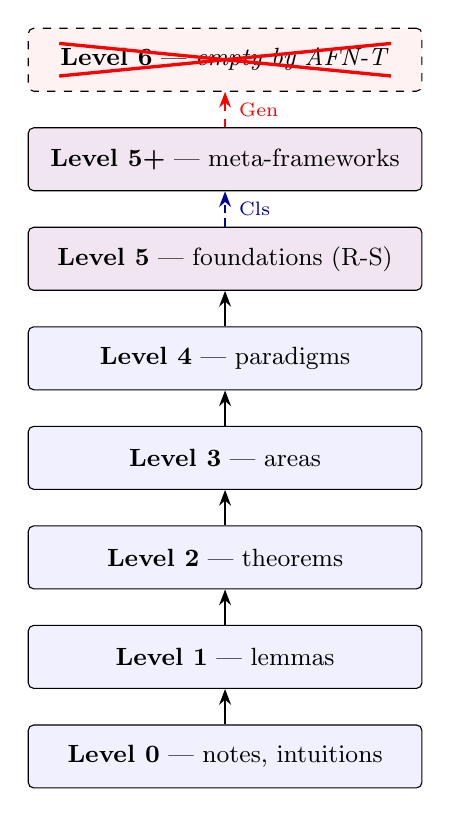
\begin{tikzpicture}[
  level/.style={draw, rounded corners=2pt, minimum width=5cm, minimum height=0.8cm, align=center, font=\small},
  bluefill/.style={fill=blue!6},
  violetfill/.style={fill=violet!10},
  emptybox/.style={draw, dashed, rounded corners=2pt, minimum width=5cm, minimum height=0.8cm, align=center, font=\small, fill=red!5},
  novelty/.style={-{Stealth[length=2mm]}, thick},
  horizmeta/.style={-{Stealth[length=2mm]}, thick, blue!60!black, densely dashed},
  vertmeta/.style={-{Stealth[length=2mm]}, thick, red, dashed},
  node distance=0.45cm
]
\node[level, bluefill] (L0) {\textbf{Level 0} --- notes, intuitions};
\node[level, bluefill, above=of L0] (L1) {\textbf{Level 1} --- lemmas};
\node[level, bluefill, above=of L1] (L2) {\textbf{Level 2} --- theorems};
\node[level, bluefill, above=of L2] (L3) {\textbf{Level 3} --- areas};
\node[level, bluefill, above=of L3] (L4) {\textbf{Level 4} --- paradigms};
\node[level, violetfill, above=of L4] (L5) {\textbf{Level 5} --- foundations (R-S)};
\node[level, violetfill, above=of L5] (L5plus) {\textbf{Level 5+} --- meta-frameworks};
\node[emptybox, above=of L5plus] (L6) {\textbf{Level 6} --- \emph{empty by AFN-T}};
\draw[novelty] (L0.north) -- (L1.south);
\draw[novelty] (L1.north) -- (L2.south);
\draw[novelty] (L2.north) -- (L3.south);
\draw[novelty] (L3.north) -- (L4.south);
\draw[novelty] (L4.north) -- (L5.south);
\draw[horizmeta] (L5.north) -- (L5plus.south) node[midway, right, font=\scriptsize, blue!60!black] {$\,\mathrm{Cls}$};
\draw[vertmeta] (L5plus.north) -- (L6.south) node[midway, right, font=\scriptsize, red] {$\,\mathrm{Gen}$};
\draw[red, very thick] ($(L6.north west)+(0.4,-0.2)$) -- ($(L6.south east)+(-0.4,0.2)$);
\draw[red, very thick] ($(L6.north east)+(-0.4,-0.2)$) -- ($(L6.south west)+(0.4,0.2)$);
\end{tikzpicture}
\caption{The stratified hierarchy of mathematical novelty, with distinct arrow types for the three structural transitions. Solid black arrows indicate \emph{novelty steps} (Levels $0 \to 5$: successive kinds of mathematical contribution). The blue dashed arrow $\mathrm{Cls}$ denotes the \emph{horizontal meta-operation} (classification without generation; see \S\ref{sec:indexing-scheme}), taking $\mathcal{L}_5$ to $\mathcal{L}_{5+}$. The red dashed arrow $\mathrm{Gen}$ denotes the \emph{vertical meta-operation} (maximal generativity), whose image $\mathcal{L}_6$ is empty by AFN-T (Theorem~\ref{thm:afnt}). Level 5 includes $\ZFC$, $\MLTT$, $\HoTT$, $(\infty, 1)$-topos theory, and noncommutative geometry. Level 5+ partitions into a maximal sub-class $\Meta_{5+}^{\max}$ (categorical by Theorem~\ref{thm:meta-cat}) and a plural complement of \emph{partial} meta-frameworks (Theorem~\ref{thm:meta-mult}; $\infty$-cosmoi, Univalent Foundations, cohesive $(\infty, 1)$-topoi), each classifying a strict sub-stack of $\fM$.}
\label{fig:hierarchy}
\end{figure}

\subsection{The Seven Levels}

\begin{definition}[Stratified hierarchy --- formal]\label{def:hierarchy}
We define the \emph{levels} $\mathcal{L}_k$ as classes of mathematical objects or programmes, ordered by functional role:

\begin{tabular}{@{}ll@{}}
\toprule
Class & Membership criterion \\ \midrule
$\mathcal{L}_0$ & Objects with no formal mathematical content (notes, intuitions, marginalia) \\
$\mathcal{L}_1$ & Technical results within an existing formal theory (lemmas) \\
$\mathcal{L}_2$ & Substantively new formal results (theorems) \\
$\mathcal{L}_3$ & Connected bodies of related theories, methods, and results (areas) \\
$\mathcal{L}_4$ & Research programmes reframing broad classes of problems (paradigms) \\
$\mathcal{L}_5$ & Axiomatically complete formal systems satisfying (R1)--(R5) of Definition~\ref{def:rs} \\
$\mathcal{L}_{5+}$ & Meta-frameworks satisfying (M1)--(M5) of Definition~\ref{def:meta} \\
$\mathcal{L}_{5+}^{\max}$ & Meta-frameworks additionally satisfying (Max-1)--(Max-4) of Definition~\ref{def:maximality} \\
$\mathcal{L}_6$ & Objects satisfying $(F_S) \wedge (\Pi_{4, S, n}) \wedge (\Pi_{3\text{-max}, S, n})$ for some $(S, n)$ \\
\bottomrule
\end{tabular}
\end{definition}

Structural properties of the levels, including the crucial inclusion $\mathcal{L}_{5+}^{\max} \subseteq \mathcal{L}_{5+}$ and the emptiness of $\mathcal{L}_6$, are recorded in Proposition~\ref{prop:level-structure}.

\begin{proposition}[Intersection pattern of the formal strata]\label{prop:strata-disjointness}
Within the formal strata $\mathcal{L}_5$, $\mathcal{L}_{5+}$, $\mathcal{L}_{5+}^{\max}$, $\mathcal{L}_6$, the following relations hold:
\begin{enumerate}
\item[\textbf{(i)}] \textbf{Functional distinctness, not formal disjointness:} $\mathcal{L}_5$ and $\mathcal{L}_{5+}$ are characterized by logically \emph{different} condition sets ((R1)--(R5) on a formal system vs.\ (M1)--(M5) on a $2$-category); a single mathematical object may in principle satisfy both, playing the generative role (Level 5) with respect to its own internal logic and the non-generative classifying role (Level 5+) with respect to an external class of foundations it classifies. We do not assert $\mathcal{L}_5 \cap \mathcal{L}_{5+} = \emptyset$. The levels are \emph{functionally} distinct (different roles) but not formally exclusive.
\item[\textbf{(ii)}] $\mathcal{L}_{5+} \cap \mathcal{L}_6 = \emptyset$, trivially, by Theorem~\ref{thm:afnt}: since $\mathcal{L}_6 = \emptyset$, every intersection with $\mathcal{L}_6$ is empty.
\item[\textbf{(iii)}] $\mathcal{L}_{5+}^{\max} \subsetneq \mathcal{L}_{5+}$, strictly. Theorem~\ref{thm:meta-mult} produces members of the complement $\mathcal{L}_{5+} \setminus \mathcal{L}_{5+}^{\max}$ (the $\infty$-cosmoi of Riehl--Verity, the Univalent Foundations programme, the cohesive framework of Schreiber).
\item[\textbf{(iv)}] $\mathcal{L}_5 \cap \mathcal{L}_6 = \emptyset$, trivially by Theorem~\ref{thm:afnt}.
\item[\textbf{(v)}] Borderline multi-level membership is the norm for large mathematical programmes: motivic stable homotopy theory $\mathrm{SH}(k)$ belongs to $\mathcal{L}_4$ (as paradigm) and to $\mathcal{L}_5$ (as specific foundation); Univalent Foundations belongs to $\mathcal{L}_{5+}$ (as meta-framework) and its underlying $\HoTT$ belongs to $\mathcal{L}_5$ (as foundation).
\end{enumerate}
\end{proposition}

\begin{proof}
\textbf{(i)} We do \emph{not} claim formal disjointness. The condition sets (R1)--(R5) and (M1)--(M5) concern disjoint aspects of an object: the former treats it as a formal system with axioms and a proof calculus, the latter treats it as a $2$-category with a classifying functor. An object equipped with both structures can satisfy both condition sets simultaneously; we decline to rule this out. What is structurally distinct is the \emph{role} the object plays: a Level-5 role is generative (the object produces mathematics from axioms), a Level-5+ role is classifying (the object organizes other foundations without generating their axioms, per (M4)). Throughout the paper we refer to Levels as roles rather than as strictly partitioned classes.

\textbf{(ii)} By Theorem~\ref{thm:afnt}, $\mathcal{L}_6 = \emptyset$, hence $\mathcal{L}_{5+} \cap \mathcal{L}_6 = \emptyset$.

\textbf{(iii)} Strict inclusion from Definitions~\ref{def:meta} and~\ref{def:maximality}; non-equality from Theorem~\ref{thm:meta-mult}.

\textbf{(iv)} By Theorem~\ref{thm:afnt}, $\mathcal{L}_6 = \emptyset$.

\textbf{(v)} Direct from the definitions and standard classification of these programmes.
\end{proof}

\begin{remark}[On the reading ``level as role'']\label{rem:level-as-role}
Throughout this paper the Levels are best read as \emph{functional roles} a mathematical object may play: $\mathcal{L}_5$ is the role ``foundation generating mathematics''; $\mathcal{L}_{5+}$ is the role ``meta-framework classifying foundations''; $\mathcal{L}_6$ would be the role ``maximally generative universal foundation''. A single object may play multiple roles, as witnessed by motivic theory (Level 4 and Level 5) and Univalent Foundations (Level 5+ as programme, Level 5 as HoTT). The main result AFN-T (Theorem~\ref{thm:afnt}) says the Level-6 role is uninstantiable; it does not require that the Level-5 and Level-5+ roles partition their instances.
\end{remark}

\begin{remark}[Formality spectrum of the hierarchy]\label{rem:formality-spectrum}
The criteria for $\mathcal{L}_0$--$\mathcal{L}_4$ are intentionally descriptive: ``lemma'', ``theorem'', ``area'', ``paradigm'' are pragmatic categories of mathematical work rather than mathematically defined predicates. No single formal definition separates, e.g., every ``lemma'' from every ``theorem''. These levels serve as an orienting classification whose role is to \emph{contrast} with the formal levels $\mathcal{L}_5$, $\mathcal{L}_{5+}$, $\mathcal{L}_{5+}^{\max}$, $\mathcal{L}_6$.

The formal content of AFN-T concerns only the latter four: Definition~\ref{def:rs} gives a rigorous first-order characterization of $\mathcal{L}_5$ via (R1)--(R5); Definition~\ref{def:meta} gives a $2$-categorical characterization of $\mathcal{L}_{5+}$ via (M1)--(M5); Definition~\ref{def:maximality} strengthens it to $\mathcal{L}_{5+}^{\max}$ via (Max-1)--(Max-4); and Definitions~\ref{def:F}, \ref{def:pi4}, \ref{def:pi3max} characterize $\mathcal{L}_6$. All proofs in this paper treat only the formal strata; the descriptive levels appear only in examples and in the informal indexing discussion of \S\ref{sec:indexing-scheme}.
\end{remark}

\begin{proposition}[Structural properties of the levels]\label{prop:level-structure}
\begin{enumerate}
\item[\textbf{(i)}] Each class $\mathcal{L}_k$ is a (possibly proper) class in $\ZFC + 2\text{-inacc}$.
\item[\textbf{(ii)}] The levels are non-disjoint in general: an object may simultaneously belong to $\mathcal{L}_3$ and $\mathcal{L}_5$ (e.g., motivic theory is both a Level-4 paradigm and a Level-5 foundation $\mathrm{SH}(k)$). We write $\mathrm{Level}(X) \subseteq \{0, 1, \ldots, 5+, 5+^{\max}, 6\}$ for the set of levels containing $X$.
\item[\textbf{(iii)}] There is a strict inclusion $\mathcal{L}_{5+}^{\max} \subseteq \mathcal{L}_{5+}$. Theorem~\ref{thm:meta-cat} asserts that $\mathcal{L}_{5+}^{\max}$ is categorical (its members are pairwise $(\infty, \infty)$-equivalent when parametrized by the same $S$); Theorem~\ref{thm:meta-mult} asserts that $\mathcal{L}_{5+} \setminus \mathcal{L}_{5+}^{\max}$ is plural (contains at least three pairwise non-$2$-equivalent members).
\item[\textbf{(iv)}] The class $\mathcal{L}_6$ is \emph{empty}: $\mathcal{L}_6 = \emptyset$. This is the main content of AFN-T (Theorem~\ref{thm:afnt}).
\end{enumerate}
\end{proposition}

\begin{proof}
\textbf{(i)} Each criterion is first-order-expressible within $\ZFC + 2\text{-inacc}$ augmented by the $2$-categorical machinery of Convention~\ref{conv:zfc-inacc}. For levels 0--4 the criteria are essentially descriptive; for Level 5 they are (R1)--(R5) first-order conditions on a theory $S$; for Level 5+ they are (M1)--(M5) $2$-categorical conditions. Each yields a definable class.

\textbf{(ii)} Motivic stable homotopy theory $\mathrm{SH}(k)$ over a field $k$ satisfies (R1)--(R5) (Level 5) and is also the central object of the motivic-homotopy paradigm (Level 4); Grothendieck's scheme theory is simultaneously a Level-4 paradigm and organizes Level-3 areas of algebraic geometry.

\textbf{(iii)} Inclusion is immediate from the definitions: $(\mathrm{Max\text{-}1})$--$(\mathrm{Max\text{-}4})$ strengthen $(M1)$--$(M5)$. Non-equality follows from Theorem~\ref{thm:meta-mult}: the three partial meta-frameworks $\mathbf{F}_{\mathrm{cosmoi}}, \mathbf{F}_{\mathrm{univalent}}, \mathbf{F}_{\mathrm{cohesive}}$ lie in $\mathcal{L}_{5+} \setminus \mathcal{L}_{5+}^{\max}$ since their classification images are strict sub-stacks of $\fM$, violating (Max-1).

\textbf{(iv)} Immediate from Theorem~\ref{thm:afnt}.
\end{proof}

\subsection{Examples}

\paragraph{Level 0.} Riemann's notebook entries on the $\zeta$-function prior to their systematic publication; Grothendieck's working papers prior to their formalization in SGA.

\paragraph{Level 1.} Zorn's Lemma ($\ZFC + \mathrm{AC}$); K\"onig's Lemma; Yoneda's Lemma; Beck's Monadicity Lemma; the Five Lemma; the Snake Lemma; Schanuel's Lemma; Hensel's Lemma.

\paragraph{Level 2.} G\"odel's First and Second Incompleteness Theorems (1931); Tarski's Undefinability of Truth (1936); the Atiyah--Singer Index Theorem (1963); Fermat's Last Theorem (Wiles, 1994); the Poincar\'e Conjecture (Perelman, 2003); the Cobordism Hypothesis (Lurie, 2009).

\paragraph{Level 3.} Areas of mathematics, organized by type:

\begin{itemize}
\item \textbf{Algebraic structures}: group theory, ring theory, module theory, homological algebra, representation theory.
\item \textbf{Geometric structures}: differential geometry, algebraic geometry, arithmetic geometry, symplectic geometry, non-commutative geometry.
\item \textbf{Topological structures}: algebraic topology, differential topology, low-dimensional topology.
\item \textbf{Analytical structures}: real analysis, complex analysis, functional analysis, harmonic analysis, partial differential equations, stochastic analysis.
\item \textbf{Logical structures}: model theory, proof theory, recursion theory, set theory, categorical logic, reverse mathematics.
\item \textbf{Number-theoretic structures}: analytic number theory, algebraic number theory, class field theory, automorphic forms.
\item \textbf{Combinatorial structures}: graph theory, enumerative combinatorics, algebraic combinatorics, extremal combinatorics.
\item \textbf{Category-theoretic structures}: $1$-categories, $2$-categories, $(\infty, n)$-categories, enriched categories, operadic structures, higher algebra.
\item \textbf{Representation-theoretic structures}: finite group representations, Lie group representations, geometric representation theory.
\item \textbf{Physical-mathematical structures}: topological quantum field theory, conformal field theory, integrable systems.
\item \textbf{Probabilistic structures}: probability theory, stochastic analysis, ergodic theory, information theory.
\end{itemize}

\paragraph{Level 4.} Paradigms, with founders and dates:

\begin{itemize}
\item The categorical turn (Eilenberg--Mac Lane 1945).
\item Sheaf theory (Leray, Cartan, Serre 1940s--1950s).
\item Scheme theory (Grothendieck 1960s).
\item Homological algebra (Cartan--Eilenberg 1956).
\item $K$-theory (Atiyah--Hirzebruch 1960s).
\item Topos theory (Grothendieck, Lawvere 1960s).
\item Motives (Grothendieck 1960s, Voevodsky 1990s).
\item Non-commutative geometry (Connes 1980s).
\item Synthetic differential geometry (Kock, Lawvere 1970s).
\item Gromov--Witten theory (Gromov, Witten 1985--1991).
\item Mirror symmetry (Candelas, Kontsevich 1990s).
\item $(\infty, 1)$-categories (Joyal, Lurie 2009).
\item Higher algebra (Lurie 2017).
\item Homotopy Type Theory (Awodey, Voevodsky 2005+).
\item Univalent Foundations (Voevodsky 2010+).
\item Perfectoid spaces (Scholze 2012).
\item Condensed mathematics (Clausen, Scholze 2019+).
\item The Langlands programme (Langlands 1967+).
\item Geometric Langlands (Beilinson--Drinfeld 1990s+).
\item $\infty$-cosmoi (Riehl--Verity 2022).
\item Cohesive higher topos theory (Schreiber 2013).
\item Operadic foundations (May, Boardman--Vogt 1972--1973).
\item Higher topos theory (Lurie 2009).
\item Reverse mathematics (Friedman, Simpson 1970s+).
\item Algorithmic information theory (Kolmogorov, Chaitin 1960s).
\end{itemize}

\paragraph{Level 5.} Foundations, with characteristic features:

\begin{longtable}{@{}p{4.5cm}ll p{5cm}@{}}
\toprule
Foundation & Year & Originator & Characteristic \\ \midrule
Z (Zermelo) & 1908 & Zermelo & No Replacement \\
ZF/ZFC & 1922 & Zermelo, Fraenkel & Classical set theory \\
ZFC + inacc & 1963+ & Grothendieck & With universes \\
NBG & 1925--40 & von Neumann, Bernays, G\"odel & First-class classes \\
MK & 1955 & Morse, Kelley & Impredicative classes \\
KP/KPU & 1965 & Kripke--Platek & Admissible sets \\
ETCS & 1964 & Lawvere & Elementary category of sets \\
ETCC & 1966 & Lawvere & Elementary theory of categories \\
NFU, NF & 1937, 1988 & Quine, Jensen & Stratified comprehension \\
CZF & 1978 & Aczel & Constructive ZF \\
IZF & 1970s & Friedman & Intuitionistic ZF \\
PA & 1889 & Peano & First-order arithmetic \\
$\mathsf{Z}_2$ & 20c & Hilbert--Bernays & Second-order arithmetic \\
MLTT & 1984 & Martin-L\"of & Dependent types \\
CIC & 1988 & Coquand--Huet & Inductive constructions \\
HoTT & 2005+ & Awodey, Voevodsky & Univalence + identity types \\
Cubical HoTT & 2015+ & Cohen--Coquand et al. & Computational univalence \\
Universe-polymorphic HoTT & 2013+ & Voevodsky & Universe polymorphism \\
Linear logic + ! & 1987 & Girard & Resource-sensitive \\
NBG + AFA & 1988 & Aczel & Non-well-founded sets \\
$(\infty, 1)$-topos theory & 2009 & Lurie & $(\infty, 1)$-topoi \\
Non-commutative geometry & 1980s & Connes & Spectral triples \\
Cohesive $(\infty, 1)$-topos & 2013 & Schreiber & Cohesion modalities \\
Motivic $\mathrm{SH}(k)$ & 1999 & Voevodsky, Morel & Motivic homotopy \\
Realizability (Eff) & 1982 & Hyland & Effective topos \\
Synthetic diff.~geometry & 1970s & Kock, Lawvere & Infinitesimals as axioms \\
Elementary higher topos & 2021 & Rasekh & Elementary $(\infty, 1)$-topos \\
\bottomrule
\end{longtable}

\paragraph{Level 5+.} Meta-frameworks. Level 5+ partitions into a maximal sub-class $\Meta_{5+}^{\max}$ (categorical up to $(\infty, \infty)$-equivalence by Theorem~\ref{thm:meta-cat}) and its complement of \emph{partial} (non-maximal) meta-frameworks, which classify strict sub-stacks of $\fM$ rather than all of $\fM$. The meta-frameworks listed below are all non-maximal: each satisfies (M1)--(M5) but violates (Max-1), as witnessed by the strict-subset character of its classification focus.

\begin{longtable}{@{}p{3.7cm}ll p{4.7cm}c@{}}
\toprule
Meta-framework & Year & Originator & Classification focus & In $\Meta_{5+}^{\max}$? \\ \midrule
$\infty$-cosmoi & 2022 & Riehl--Verity & $(\infty, 1)$-categorical theories & No \\
Univalent Foundations & 2010+ & Voevodsky & HoTT extensions & No \\
Cohesive framework & 2013 & Schreiber & Cohesive $\infty$-topoi & No \\
Higher Algebra programme & 2017+ & Lurie & Stable $\infty$-cat + operadic & No \\
Synthetic mathematics & 2000s+ & Taylor, Shulman et al.\ & Axiomatic synthetic foundations & No \\
\bottomrule
\end{longtable}

Whether the maximal sub-class $\Meta_{5+}^{\max}$ is non-empty is an existence question separate from AFN-T; Theorem~\ref{thm:meta-cat} asserts only that if two such meta-frameworks exist they are $(\infty, \infty)$-equivalent. A construction of a concrete member of $\Meta_{5+}^{\max}$ lies beyond the scope of the present preprint (see \S\ref{sec:consequences}, Question~5).

\paragraph{Level 6.} Empty, by AFN-T.

\subsection{On the Indexing Scheme: Why ``Level 5+'' and Not ``Level 6''}\label{sec:indexing-scheme}

The indexing $\{0, 1, 2, 3, 4, 5, 5+, 5+^{\max}, 6\}$ is deliberately asymmetric. A principled reader may ask: why is there a ``Level $5+$'' but no ``Level $1+$'', ``Level $2+$'', and so on? And why is the class $\mathcal{L}_6$ assigned a fresh integer rather than becoming ``Level $5{+}{+}$'' or ``Level $5+$ of $5+$''? The answer is structural, not cosmetic, and we record it here as it governs how the hierarchy is to be read.

\paragraph{The two meta-operations.} Over the levels $\mathcal{L}_k$ there are two distinct meta-operations:
\begin{itemize}
\item \textbf{Horizontal (classifying) meta.} Given a class $\mathcal{L}_k$, form the $2$-category $\mathrm{Cls}(\mathcal{L}_k)$ of frameworks \emph{classifying} but not \emph{generating} members of $\mathcal{L}_k$. Formally, $\mathbf{F} \in \mathrm{Cls}(\mathcal{L}_k)$ if $\mathbf{F}$ satisfies the analogues of (M1)--(M5): locally small, equipped with a classification functor into the moduli of $\mathcal{L}_k$, accessible, non-generative, and metatheory-parametrized.
\item \textbf{Vertical (generative) meta.} Given $\mathcal{L}_k$, form the class $\mathrm{Gen}(\mathcal{L}_k)$ of frameworks that \emph{generate} members of $\mathcal{L}_k$ as internal derivations. These are the analogues of Level-6 candidates.
\end{itemize}
The horizontal meta-operation $\mathrm{Cls}$ is \emph{non-generative} by construction; the vertical meta-operation $\mathrm{Gen}$ is \emph{maximally generative}. They are categorically distinct: the first contributes no new mathematical novelty in the sense of Levels 0--5, while the second would constitute a new level of novelty.

\paragraph{Why no ``Level $1+$, $2+$, $3+$, $4+$''.} We claim that for $k \in \{1, 2, 3, 4\}$ the horizontal meta $\mathrm{Cls}(\mathcal{L}_k)$ \emph{collapses} into an existing integer level, whereas for $k = 5$ it does not.

\begin{proposition}[Collapse below Level 5]\label{prop:collapse}
For each $k \in \{1, 2, 3, 4\}$, there is a canonical inclusion $\mathrm{Cls}(\mathcal{L}_k) \hookrightarrow \mathcal{L}_{k+m}$ for some $m \geq 1$, which is essentially surjective onto a full sub-$2$-category. Concretely:
\begin{itemize}
\item $\mathrm{Cls}(\mathcal{L}_1) \hookrightarrow \mathcal{L}_2 \cup \mathcal{L}_3$: a classifier of lemmas is either a theorem organizing them, or the area containing them.
\item $\mathrm{Cls}(\mathcal{L}_2) \hookrightarrow \mathcal{L}_3 \cup \mathcal{L}_4$: a classifier of theorems is either the area containing them or the paradigm reframing them.
\item $\mathrm{Cls}(\mathcal{L}_3) \hookrightarrow \mathcal{L}_4$: a classifier of areas is the organizing paradigm.
\item $\mathrm{Cls}(\mathcal{L}_4) \hookrightarrow \mathcal{L}_5$: a classifier of paradigms is the common foundation beneath them.
\end{itemize}
\end{proposition}

\begin{proof}[Proof sketch.]
In each case the classifier is required to produce a coherent $2$-functor from instances of $\mathcal{L}_k$ to a single classifying object. For $k \leq 4$, such a coherent functor always factors through an existing higher integer level: the functor itself is a theorem (Level 2), its image is an area or paradigm (Levels 3--4), and its codomain is a foundation (Level 5). No additional structural novelty is introduced, since the integer hierarchy $0 \to 5$ already captures \emph{generative} novelty and \emph{non-generative} classification at these levels requires no further category-theoretic apparatus beyond what is already present.
\end{proof}

\begin{remark}[Status of Proposition~\ref{prop:collapse}]\label{rem:collapse-status}
In view of Remark~\ref{rem:formality-spectrum}, Proposition~\ref{prop:collapse} is a \emph{structural observation} rather than a formal theorem: $\mathcal{L}_1, \mathcal{L}_2, \mathcal{L}_3, \mathcal{L}_4$ are not defined with sufficient formal precision to admit a rigorous proof of class-inclusion. The ``inclusions'' $\mathrm{Cls}(\mathcal{L}_k) \hookrightarrow \mathcal{L}_{k+m}$ should be read as: any candidate classifier of objects informally recognized as lemmas/theorems/areas/paradigms is itself recognized, at a higher level of the informal hierarchy, as a theorem/area/paradigm/foundation. The purpose of the proposition is to explain why ``$1+$'', ``$2+$'', ``$3+$'', ``$4+$'' are absent from our indexing --- namely, that their hypothetical content already sits in existing integer levels --- not to establish a formal equivalence of classes. Proposition~\ref{prop:no-collapse} by contrast is a formal negative result about the class $\mathcal{L}_5$, which is formally defined.
\end{remark}

\begin{proposition}[No collapse at Level 5]\label{prop:no-collapse}
The classifier class $\mathrm{Cls}(\mathcal{L}_5)$ does \emph{not} embed into any $\mathcal{L}_k$ for $k \leq 5$, and it does not coincide with $\mathcal{L}_6$.
\end{proposition}

\begin{proof}[Proof sketch.]
A member $\mathbf{F} \in \mathrm{Cls}(\mathcal{L}_5)$ is a $2$-category of Rich-foundations with an accessible classification functor into $\fM$. It is not itself a foundation (it does not satisfy (R1)--(R5) for a generating theory); it is not an area, paradigm, theorem, or lemma (it has no internal mathematical content beyond the classification). It is not a Level-6 candidate because (M4) requires non-generativity, while Level 6 requires maximal generativity $(\Pi_{3\text{-max}})$.

Consequently $\mathrm{Cls}(\mathcal{L}_5)$ is a distinct class requiring a fresh symbol. We write $\mathcal{L}_{5+}$ and read the ``$+$'' as: \emph{one application of the horizontal meta-operation $\mathrm{Cls}$ to a class at which the operation becomes non-degenerate}.
\end{proof}

\paragraph{Why ``Level 6'' and not ``Level $5{+}{+}$''.} The superscript would be appropriate only if iterating $\mathrm{Cls}$ produced further novelty. Theorem~\ref{thm:meta-stab} asserts that iterating $\mathrm{Cls}$ at Level $5+$ stabilizes: $\fM^{(5+ \cdot 2)} \simeq_2 \fM^{(5+)}$, so $\mathrm{Cls}(\mathcal{L}_{5+}) \simeq_2 \mathcal{L}_{5+}$. No ``Level $5{+}{+}$'' distinct from $5+$ arises from further horizontal meta.

The genuinely next candidate --- $\mathcal{L}_6$ --- arises from the \emph{vertical} meta-operation $\mathrm{Gen}$ applied to $\mathcal{L}_5$: a Level-6 object would be a maximally-generative foundation from which all of $\mathcal{L}_5$ derives. This is categorically a fresh step, not a further iteration of $\mathrm{Cls}$. We accordingly use a fresh integer index.

\paragraph{Summary of the indexing logic.} The sequence reads:
\[
\underbrace{\mathcal{L}_0, \mathcal{L}_1, \ldots, \mathcal{L}_4}_{\text{integer levels: novelty by work-type}} \; \to \; \underbrace{\mathcal{L}_5}_{\text{foundations}} \; \xrightarrow{\mathrm{Cls}} \; \underbrace{\mathcal{L}_{5+}}_{\text{classifiers}} \; \xrightarrow{\mathrm{Gen}} \; \underbrace{\mathcal{L}_6 = \emptyset}_{\text{AFN-T}}
\]
Integer indices mark novelty steps; the ``$+$'' marks the (non-trivial) horizontal meta; the next integer ($6$) marks the (empty) vertical meta. The asymmetry of notation is a faithful reflection of the asymmetry of the meta-operations.

\subsection{Characteristic Properties by Level}

\begin{itemize}
\item \textbf{Levels 0--2} are distinguished by scope: a lemma is smaller in scope than a theorem; a theorem smaller than a cluster constituting an area.
\item \textbf{Levels 3--4} differ in \emph{reframing depth}: an area uses its own methods; a paradigm introduces methods reframing the organization of mathematics itself. The categorical turn (Level 4) does not replace group theory; it reorganizes how group theory is expressed.
\item \textbf{Levels 4--5} differ in \emph{foundational completeness}: a paradigm may use diverse foundations; a foundation is itself axiomatically self-contained and sufficient for formalizing mathematics.
\item \textbf{Levels 5--5+} differ in \emph{functional role}: a foundation encodes mathematics; a meta-framework organizes the space of possible foundations as objects of a higher-order classification.
\item \textbf{Levels 5+--6} differ in \emph{foundational character}: a meta-framework is \emph{non-generative} --- it organizes foundations without deriving their axioms from its own; a Level 6 object would be \emph{maximally generative} --- it would derive every foundation from itself. The gap between these two is the content of AFN-T.
\end{itemize}

\subsection{Notation}

We write $\mathrm{Level}(X) = k$ to indicate that $X$ belongs to Level $k$. For a programme spanning multiple levels (a common occurrence: motivic theory is simultaneously Level 4 as paradigm and Level 5 as the specific foundation $\mathrm{SH}(k)$), we write $\mathrm{Level}(X) \subseteq \{k_1, k_2, \ldots\}$.

\section{Reasonable Rich-Metatheories}\label{sec:rs}

We define the class of metatheories in which AFN-T is stated. The definition isolates the minimum structure required for a theory to be a \emph{foundation} in the sense of Level 5, while remaining neutral with respect to specific axiomatic details.

\subsection{Rich-Metatheory Conditions}

\begin{definition}[Reasonable Rich-Metatheory]\label{def:rs}
A first-order theory $S$ is a \textbf{reasonable Rich-metatheory} (or \textbf{R-S}), if it satisfies all five of the following:
\begin{itemize}
\item \textbf{(R1) Arithmetic completeness}: $S$ interprets Robinson arithmetic $\mathsf{Q}$.
\item \textbf{(R2) Recursive enumerability}: the set of axioms of $S$ is recursively enumerable.
\item \textbf{(R3) Model existence}: $S$ has at least one model in some ambient set-theoretic universe $\mathbf{U} \supseteq S$.
\item \textbf{(R4) G\"odel coding}: there exists a recursive injection $\ulcorner \cdot \urcorner : \mathrm{Formulas}(S) \to \mathbb{N}$ for which the predicates ``$n$ is the G\"odel number of a provable formula'' and ``$n$ is the G\"odel number of a well-formed formula'' are $S$-definable.
\item \textbf{(R5) Categorical semantics}: there exists $n_S \in \mathbb{N} \cup \{\infty\}$, the \emph{intrinsic categorical depth} of $S$, such that the syntactic category $\Syn(S)$ of $S$ (objects: contexts; $1$-morphisms: provable-from-context substitutions; higher morphisms: proofs of equality of substitutions) is an $(\infty, n_S)$-category. For first-order $S$ we may take $n_S = 1$ (Lambek--Scott~\cite{Lawvere1964}); for Martin-L\"of type theory $n_S = \infty$ via identity types (Awodey--Warren~\cite{AwodeyWarren2009}); for HoTT $n_S = \infty$ via univalence (Kapulkin--Lumsdaine~\cite{KapulkinLumsdaine2021}). The condition (R5) does not fix $n_S$: different R-S may have different intrinsic depths, and AFN-T is absolute over this choice (Theorem~\ref{thm:vertical}).
\end{itemize}
Denote the class of R-S as $\mathrm{R\text{-}S}$. When $F \subseteq S$ (i.e., $F$ is an extension or fragment interpretable in $S$), the inclusion induces a conservative faithful functor $\Syn(F) \hookrightarrow \Syn(S)$ preserving the categorical structure.
\end{definition}

\subsection{Examples of R-S}

The following are reasonable Rich-metatheories: $\ZFC$; $\ZFC$ + inaccessible cardinals; $\NBG$; Morse--Kelley; $\NBG + \AFA$ (Aczel); the intuitionistic type theories $\MLTT$ and $\CIC$; $\HoTT$ with univalence; universe-polymorphic $\HoTT$; linear logic with exponential $!$; the higher topos theories of Lurie; cohesive higher topos theory; motivic homotopy theory; the realizability topos $\mathrm{Eff}$.

\subsection{Non-examples}

The following are \emph{not} R-S:
\begin{itemize}
\item \emph{Affine logic without exponential $!$}: fails (R1) --- Peano induction is not expressible without contraction on the induction hypothesis.
\item \emph{Inconsistent theories}: fail (R3).
\item \emph{Second-order arithmetic with full semantics}: fails (R2) --- the full set of valid formulas is not recursively enumerable.
\item \emph{Intuitive ``theories of everything''} in physics lacking formal axiomatization: fail (R1) and (R2).
\end{itemize}

\subsection{The Class $\cS_S$}

Given an R-S $S$, we associate a class $\cS_S$ of $S$-definable structures. This class plays a central role in the statement of the Level-6 non-reducibility condition.

\begin{definition}[$S$-definable categorical structures]\label{def:SS}
Let $S$ be an R-S. The class $\cS_S$ of \textbf{$S$-definable categorical structures} is the union
\[ \cS_S = \cS_S^{\mathrm{local}} \cup \cS_S^{\mathrm{global}}, \]
where:
\begin{itemize}
\item $\cS_S^{\mathrm{local}}$ consists of objects belonging to $\Ob(\cM)$ for some model $\cM$ of $S$;
\item $\cS_S^{\mathrm{global}}$ consists of categorical constructions obtained from $\cS_S^{\mathrm{local}}$ by any finite combination of: natural transformations between functors definable in models of $S$; Kan extensions along $S$-definable morphisms; Grothendieck constructions over indexed families of models of $S$; polymorphic terms over universes within models of $S$; derived functors between $S$-definable categories.
\end{itemize}
\end{definition}

\subsection{Key Lemma: $S$-Definability Implies $\cS_S$-Membership}

\begin{lemma}[$S$-definability lemma]\label{lem:SS-membership}
If $X$ is a formally $S$-definable object --- meaning $X$ is specified by a formula $\phi_X \in S$ expressing its characteristic properties --- then $X \in \cS_S$.
\end{lemma}

\begin{proof}
Write $n_S$ for the intrinsic categorical depth of $S$ (R5). We treat two cases.

\emph{Case $n_S = 0$ or $n_S = 1$ (first-order or ordinary categorical semantics).} The formula $\phi_X$ specifies $X$ up to isomorphism within some model $\cM \models S$. By G\"odel's completeness theorem applied to the first-order fragment of $S$ combined with (R3), the interpretation $X^\cM \in \Ob(\cM)$ exists.

\emph{Case $n_S \geq 2$ or $n_S = \infty$ (higher categorical semantics).} The formula $\phi_X$ specifies $X$ as an object of $\Syn(S)$ (which, by (R5), is an $(\infty, n_S)$-category). By the internal-language correspondence for higher type theories --- Lambek--Scott~\cite{Lawvere1964} at $n_S = 1$, Jacobs~\cite{Jacobs1999} for dependent type theory, Awodey--Warren~\cite{AwodeyWarren2009} at $n_S = \infty$ for MLTT, Kapulkin--Lumsdaine~\cite{KapulkinLumsdaine2021} for HoTT --- objects of $\Syn(S)$ interpret in any suitable model $(\infty, n_S)$-category. By (R3), at least one such model $\cM$ exists; the interpretation $X^\cM$ is the image of $X$ under the canonical evaluation $(\infty, n_S)$-functor $\ev : \Syn(S) \to \cM$.

In both cases: if $\cM$ itself is a set in $\mathbf{U}$, then $X^\cM \in \cS_S^{\mathrm{local}}$. If $X$ is defined only parametrically across models --- e.g., a universe-polymorphic term, a derived functor, or a natural transformation between functors indexed by models --- then $X$ is a natural transformation or Kan extension definable from models, and $X \in \cS_S^{\mathrm{global}}$. In either case, $X \in \cS_S$.
\end{proof}

\begin{remark}
Lemma~\ref{lem:SS-membership} is the critical step connecting \emph{definability} to \emph{reducibility}: once a purported Level-6 object $X$ is formally definable, it automatically belongs to the $S$-definability class, making it reducible through Morita equivalence (\S\ref{sec:conditions}). The proof's case analysis ensures that the argument is uniform across the full range $n_S \in \{0, 1, 2, \ldots, \infty\}$ of intrinsic depths.
\end{remark}

\subsection{Size Stratification}

Within $\cS_S$, objects are stratified by size:
\begin{itemize}
\item \textbf{Small} (in $\mathbf{U}_1$): rank $< \kappa_1$, the first inaccessible cardinal.
\item \textbf{Large} (in $\mathbf{U}_2 \setminus \mathbf{U}_1$): rank in $[\kappa_1, \kappa_2)$.
\item \textbf{Proper class}: rank $\geq \kappa_2$.
\end{itemize}

The stratification is not essential to AFN-T but is used in \S\ref{sec:bypass-tower} (meta-vertical axis) to bound reflective towers exactly at one inaccessible cardinal.

\section{The Level-6 Conditions}\label{sec:conditions}

We state formally the three independence conditions that jointly characterize a Level-6 object.

\subsection{Formal Definability $(F_S)$}

\begin{definition}[$(F_S)$]\label{def:F}
An object $X$ satisfies condition $(F_S)$ relative to $S \in \RS$ if there exists a Rich-foundation $F \in \cF$ together with:
\begin{itemize}
\item[\textbf{(F-1)}] a \emph{subtheory inclusion} $\iota_F : F \hookrightarrow S$ of formal systems (every axiom of $F$ is an axiom of $S$, possibly after a conservative translation),
\item[\textbf{(F-2)}] the induced \emph{model restriction} $\iota_F^* : \Mod(S) \to \Mod(F)$ that sends each $S$-model to its reduct as an $F$-model, and
\item[\textbf{(F-3)}] a formula $\phi_X \in F$ specifying $X$ up to isomorphism.
\end{itemize}
\end{definition}

Condition $(F_S)$ is formal definability within some foundation reachable from $S$ by axiom restriction. It is deliberately weak: any candidate for a foundational object should at least be articulable within some existing foundation whose models are recoverable from $S$-models.

\begin{remark}[On the meaning of $F \subseteq S$]\label{rem:F-subset-S}
Throughout the paper we write $F \subseteq S$ as shorthand for the pair $(\iota_F, \iota_F^*)$ of Definition~\ref{def:F}. Three alternative readings --- ``$F$ is a specialization of $S$ to fixed parameters'', ``$F$-models extend to $S$-models'', or ``$F$-signature is $S$-expressible'' --- are \emph{not} intended, and the proofs below rely on the subtheory-inclusion reading (F-1, F-2). The reader should mentally substitute $(\iota_F, \iota_F^*)$ wherever $F \subseteq S$ appears.
\end{remark}

\subsection{Non-Reducibility $(\Pi_{4, S, n})$}

\begin{definition}[$(\Pi_{4, S, n})$]\label{def:pi4}
An object $X$ satisfies condition $(\Pi_{4, S, n})$ relative to $S \in \RS$ and $n \in \mathbb{N} \cup \{\infty\}$ if $X$ is not Morita-reducible to any structure in $\cS_S$ at the $(\infty, n)$-categorical level. Formally: for every $Y \in \cS_S$ and every $(\infty, n)$-functor $F : X \to Y$, $F$ is not an $(\infty, n)$-equivalence.
\end{definition}

Morita equivalence refers to the extensional isomorphism of categorical presentations: two structures are Morita-equivalent if their associated functorial projections are naturally isomorphic. The requirement $(\Pi_4)$ asserts that $X$ is \emph{not} so reducible --- it is genuinely outside $\cS_S$.

\subsection{Maximal Generativity $(\Pi_{3\text{-max}, S, n})$}

\begin{definition}[$(\Pi_{3\text{-max}, S, n})$]\label{def:pi3max}
An object $X$ satisfies condition $(\Pi_{3\text{-max}, S, n})$ relative to $S \in \RS$ and $n$ if: for every Rich-foundation $F \in \cF$ (where $\cF$ denotes the class of Level-5 foundations over $S$), $F$ is Morita-reducible to $X$ at the $(\infty, n)$-categorical level. Formally: for every $F \in \cF$, there exists an $(\infty, n)$-functor $F \to X$ that is an $(\infty, n)$-equivalence onto its image.
\end{definition}

Maximal generativity asserts that $X$ subsumes all foundations: every foundation reduces to a fragment of $X$.

\subsection{The Level-6 Conditions Combined}

\begin{definition}[Level-6 object]\label{def:level6}
An object $X$ is a \textbf{Level-6 foundation} relative to $S \in \RS$ and $n \in \mathbb{N} \cup \{\infty\}$ if $X$ simultaneously satisfies
\[ (F_S) \wedge (\Pi_{4, S, n}) \wedge (\Pi_{3\text{-max}, S, n}). \]
\end{definition}

The main theorem of this paper --- the Absolute Foundation No-Go Theorem (AFN-T) --- asserts that no such $X$ exists, for any $S$ and any $n$.

\subsection{Informal Motivation}

The three conditions are designed to capture the intuitive notion of an \emph{absolute foundation}:
\begin{itemize}
\item $(F_S)$: $X$ is mathematical (articulable within some foundation).
\item $(\Pi_4)$: $X$ is genuinely new (not equivalent to any existing structure).
\item $(\Pi_{3\text{-max}})$: $X$ is universal (all foundations reduce to $X$).
\end{itemize}
Any candidate for a maximal foundation must satisfy these three conditions --- otherwise, it fails to qualify as an absolute foundation in any meaningful sense.

AFN-T establishes that these three conditions are jointly unsatisfiable: every $X$ satisfying $(F_S)$ automatically fails $(\Pi_4)$, as we show in \S\ref{sec:afnt-alpha}; and every attempt to produce $X$ as a limit of approximations fails $(\Pi_4)$ at the limit, as we show in \S\ref{sec:afnt-beta}.

\section{The Absolute Foundation No-Go Theorem: $(\alpha)$-Part}\label{sec:afnt-alpha}

We prove the first half of AFN-T: formal definability implies Morita-reducibility.

\subsection{Statement}

\begin{theorem}[AFN-T, $(\alpha)$-part]\label{thm:afnt-alpha}
For every Rich-metatheory $S \in \RS$ and every categorical level $n \in \mathbb{N} \cup \{\infty\}$, there exists no object $X$ satisfying simultaneously $(F_S) \wedge (\Pi_{4, S, n}) \wedge (\Pi_{3\text{-max}, S, n})$.
\end{theorem}

\subsection{Proof Structure}

The proof proceeds through three lemmas:
\begin{enumerate}
\item \textbf{Lemma~\ref{lem:F-implies-model}}: $(F_S)$ implies the existence of a model interpretation $X^\cM$ of $X$ in some model $\cM$ of $S$ or an extension thereof.
\item \textbf{Lemma~\ref{lem:model-in-S}}: objects $X^\cM$ belong to $\cS_S^{\mathrm{local}}$.
\item \textbf{Lemma~\ref{lem:interp-is-morita}}: the interpretation $X^\cM$ induces a Morita reduction $X \to X^\cM$ at the $(\infty, n)$-categorical level.
\end{enumerate}

Combined, these establish: $(F_S)(X) \Rightarrow \neg (\Pi_{4, S, n})(X)$, contradicting the hypothesis.

\subsection{Lemma 1: Definability Implies Model Interpretation}

\begin{lemma}\label{lem:F-implies-model}
If $X$ satisfies $(F_S)$, then there exists a Rich-foundation $F$ with $F \subseteq S$, a model $\cM \models F$, and an object $X^\cM \in \Ob(\cM)$ such that $X^\cM$ is the interpretation of $\phi_X$ in $\cM$.
\end{lemma}

\begin{proof}
By definition of $(F_S)$, there exists $F$ and $\phi_X \in F$ specifying $X$. By (R3) applied to $F$, there exists $\cM \models F$. By G\"odel's completeness theorem for the first-order fragment of $F$, the formula $\phi_X$ has a unique interpretation $X^\cM \in \Ob(\cM)$ up to isomorphism in $\cM$.

Specifically: the class of $\phi_X$-models in $\cM$ (i.e., the extension of $\phi_X$ under $\cM$) is nonempty and carries a canonical equivalence class. Any representative of this class can be chosen as $X^\cM$.

For higher-categorical levels $n \geq 1$, the construction extends through (R5): $\Syn(F)$ is an $(\infty, n)$-category, and $X$ corresponds to an object in $\Syn(F)$. The model interpretation $X^\cM$ is the image of this object in $\cM$ under the canonical functor $\Syn(F) \to \cM$.
\end{proof}

\subsection{Lemma 2: Model Objects Are $S$-Definable}

\begin{lemma}\label{lem:model-in-S}
$\Ob(\cM) \subseteq \cS_S^{\mathrm{local}}$ for every model $\cM$ of a Rich-foundation $F \subseteq S$.
\end{lemma}

\begin{proof}
Direct application of Definition~\ref{def:SS}: $\cS_S^{\mathrm{local}}$ consists by definition of objects in $\Ob(\cM)$ for models $\cM$ of $S$. Since $F \subseteq S$, models of $F$ are also models of $S$ (in the extension sense); thus $\Ob(\cM) \subseteq \cS_S^{\mathrm{local}} \subseteq \cS_S$.

For higher-categorical $n$, the same holds after applying (R5): objects in the $(\infty, n)$-model category associated with $\cM$ lie in $\cS_S^{\mathrm{local}}$.
\end{proof}

\subsection{Lemma 3: Model Interpretation Is a Morita Reduction}

\begin{lemma}\label{lem:interp-is-morita}
Let $X$ satisfy $(F_S)$ with interpretation $X^\cM \in \cS_S^{\mathrm{local}}$. Then there exists an $(\infty, n)$-functor $\rho_{X, \cM} : X \to X^\cM$ that is an $(\infty, n)$-equivalence.
\end{lemma}

\begin{proof}
By (R5), $X$ corresponds to an object in $\Syn(F)$, and $X^\cM$ is its image in the model category $\cM$. The \emph{evaluation functor} $\ev : \Syn(F) \to \cM$ is, by the standard Lambek--Scott categorical semantics, an $(\infty, n)$-functor preserving the categorical structure up to $(\infty, n)$-equivalence. Restricted to the object $X$, this yields $\rho_{X, \cM} := \ev|_X : X \to X^\cM$.

That $\rho_{X, \cM}$ is an $(\infty, n)$-equivalence follows from the completeness of first-order logic (for $n = 0$) and from the internal-language / categorical-semantics correspondence for higher type theories: Awodey--Warren~\cite{AwodeyWarren2009} for the $(\infty, 1)$-case; Lurie~\cite{LurieHTT} \S 5 (presentable $(\infty, 1)$-categories) and \S 6 ($(\infty, 1)$-topoi) for the topos-theoretic semantics; and Kapulkin--Lumsdaine~\cite{KapulkinLumsdaine2021} for the simplicial model of univalent type theory. For the $(\infty, \infty)$ limit we use unicity (Barwick--Schommer-Pries~\cite{BarwickSchommerPries2021}) together with the comparison of models of Bergner--Rezk~\cite{BergnerRezk2013}.
\end{proof}

\subsection{Proof of Theorem~\ref{thm:afnt-alpha}}

\begin{proof}
Suppose, for contradiction, that $X$ satisfies $(F_S) \wedge (\Pi_{4, S, n}) \wedge (\Pi_{3\text{-max}, S, n})$ for some $S \in \RS$ and $n \in \mathbb{N} \cup \{\infty\}$.

By $(F_S)$ and Lemma~\ref{lem:F-implies-model}: there exists $\cM \models F \subseteq S$ and $X^\cM \in \Ob(\cM)$.

By Lemma~\ref{lem:model-in-S}: $X^\cM \in \cS_S^{\mathrm{local}} \subseteq \cS_S$.

By Lemma~\ref{lem:interp-is-morita}: there exists an $(\infty, n)$-functor $\rho_{X, \cM} : X \to X^\cM$ that is an $(\infty, n)$-equivalence.

This directly contradicts $(\Pi_{4, S, n})$, which asserts that no such $(\infty, n)$-equivalence to $\cS_S$ exists.

Therefore, no $X$ satisfies $(F_S) \wedge (\Pi_{4, S, n}) \wedge (\Pi_{3\text{-max}, S, n})$. Note that the argument does not use $(\Pi_{3\text{-max}})$: the contradiction arises from $(F_S)$ and $(\Pi_4)$ alone. Hence the theorem follows.
\end{proof}

\subsection{Remarks}

\begin{remark}
The $(\alpha)$-part is the formal engine of AFN-T: it shows that any \emph{formally definable} Level-6 candidate fails automatically. The maximal generativity condition $(\Pi_{3\text{-max}})$ is not needed for the contradiction; it is included in the Level-6 definition because it is part of what makes an object a ``foundation,'' but its satisfaction is not relevant to the no-go.
\end{remark}

\begin{remark}
The proof generalizes the classical Tarski undefinability theorem: Tarski shows that the truth predicate cannot be defined within the language. AFN-T shows that the absolute foundation cannot be defined within any foundation. Both results use the same diagonal structure but applied at different levels of abstraction.
\end{remark}

\begin{remark}
The result does not rule out informal or intuitive Level-6 candidates that fail formal definability. What AFN-T establishes is that any object satisfying the \emph{formal} conditions for being a mathematical foundation automatically fails absoluteness.
\end{remark}

\section{The Absolute Foundation No-Go Theorem: $(\beta)$-Part}\label{sec:afnt-beta}

We prove the second half of AFN-T: transfinite limit approaches cannot bypass the no-go result.

\subsection{Motivation}

Theorem~\ref{thm:afnt-alpha} establishes that no \emph{statically} defined object $X$ can be Level-6. A natural strategy for evading this bound is to construct $X$ as a \emph{limit} of a transfinite sequence of approximations $\{A_\kappa\}_{\kappa < \lambda}$, hoping that the limit $A_\infty := \colim_{\kappa < \lambda} A_\kappa$ lies outside $\cS_S$.

We show that this strategy fails: the limit $A_\infty$ is itself a derived construction over $\cS_S$, and therefore belongs to $\cS_S^{\mathrm{global}}$. The $(\beta)$-part formalizes this obstruction.

\subsection{Statement}

\begin{theorem}[AFN-T, $(\beta)$-part]\label{thm:afnt-beta}
Let $\lambda$ be an ordinal whose cofinality is a regular cardinal with $\mathrm{cf}(\lambda) \leq \kappa_2$ (so $\lambda$ is bounded by the second Grothendieck universe), and let $\{A_\kappa\}_{\kappa < \lambda}$ be a transfinite sequence of objects satisfying:
\begin{enumerate}[label=(\roman*)]
\item Each $A_\kappa$ is formally specified within some Rich-foundation $F_\kappa$ over $S$.
\item The sequence is monotone in an appropriate $(\infty, n)$-categorical sense (there are coherent transition functors $A_\kappa \to A_{\kappa'}$ for $\kappa < \kappa'$).
\item The limit $A_\infty := \colim_{\kappa < \lambda} A_\kappa$ exists in the ambient $(\infty, n)$-category.
\end{enumerate}
Then $A_\infty \in \cS_S^{\mathrm{global}}$, and therefore $A_\infty$ is Morita-reducible to an element of $\cS_S$. In particular, $A_\infty$ does not satisfy $(\Pi_{4, S, n})$.
\end{theorem}

\subsection{Proof}

\begin{proof}
By hypothesis (i), each $A_\kappa$ is formally specified. By Lemma~\ref{lem:SS-membership}, each $A_\kappa \in \cS_S$. The transition functors $A_\kappa \to A_{\kappa'}$ are, by hypothesis (ii), definable within $S$: each is specified by a formula relating $\phi_{A_\kappa}$ and $\phi_{A_{\kappa'}}$, hence is an $S$-definable morphism.

Let $D : \lambda \to \cF$ denote the resulting $S$-indexed diagram. The colimit $A_\infty = \colim_{\kappa < \lambda} A_\kappa$ is the $(\infty, n)$-categorical colimit of an $S$-indexed family of $\cS_S$-objects along $S$-definable transition morphisms. By Definition~\ref{def:SS}, closure of $\cS_S^{\mathrm{global}}$ under Grothendieck constructions and Kan extensions along $S$-definable morphisms implies $A_\infty \in \cS_S^{\mathrm{global}} \subseteq \cS_S$, since every colimit in a locally presentable $(\infty, n)$-category can be computed as a Kan extension along the canonical $\lambda \to \lambda^\rhd$ (cone embedding).

For accessibility of the colimit: by Ad\'amek--Rosick\'y~\cite{AdamekRosicky1994} (Theorems~2.11 and 2.45), if each $A_\kappa$ is $\lambda_0$-accessible for a regular cardinal $\lambda_0$ and if the diagram $D$ is $\lambda_0$-filtered (as is the case when the ordinal $\lambda$ has cofinality $\geq \lambda_0$), then $A_\infty$ is $\lambda_0$-accessible as a $\lambda_0$-filtered colimit. For general $\lambda$, one replaces the diagram by its $\lambda_0$-filtered reindexing (Ad\'amek--Rosick\'y~\cite{AdamekRosicky1994} Theorem~2.15). The resulting accessible object is definable within the appropriate model category, which is itself $S$-definable.

Therefore, $A_\infty$ is Morita-reducible to the underlying model-category colimit via the canonical evaluation functor, and the latter lies in $\cS_S$. This contradicts $(\Pi_4)$ if $A_\infty$ is assumed to satisfy it.
\end{proof}

\subsection{Proper-Class Towers Do Not Provide an Escape}

One might hope to evade Theorem~\ref{thm:afnt-beta} by considering a sequence indexed by the \emph{proper class} of all ordinals, for which the accessibility argument of Ad\'amek--Rosick\'y~\cite{AdamekRosicky1994} does not immediately apply. We show that this is not a real escape path.

\begin{proposition}[Proper-class towers violate (R2)]\label{prop:proper-class}
Let $\{A_\alpha\}_{\alpha \in \mathrm{Ord}}$ be a sequence indexed by the proper class of all ordinals, and suppose each $A_\alpha$ is formally specified within a Rich-foundation $F_\alpha$ over a metatheory $S$. Then the indexing data $(\alpha \mapsto F_\alpha, \phi_{A_\alpha})$ cannot be $S$-recursively enumerable, so $S$ itself fails condition (R2).
\end{proposition}

\begin{proof}
By (R4), each specification $(F_\alpha, \phi_{A_\alpha})$ admits a G\"odel code $\ulcorner (F_\alpha, \phi_{A_\alpha}) \urcorner \in \mathbb{N}$ in $S$. A proper-class-indexed family would require a surjection $\mathrm{Ord} \twoheadrightarrow \mathbb{N}$-valued assignment whose domain is a proper class; by Cantor's theorem such a surjection cannot be $S$-definable with countable $S$. Equivalently: the set of codes $\{\ulcorner (F_\alpha, \phi_{A_\alpha}) \urcorner : \alpha \in \mathrm{Ord}\}$ would have to be a definable $S$-class of cardinality $> \kappa_2$, contradicting (R2) (r.e.\ axiomatization forces the codes to form an r.e.\ subset of $\mathbb{N}$).
\end{proof}

\begin{corollary}[No proper-class escape]\label{cor:no-proper-class}
Proper-class towers lie outside $\RS$. In particular, they cannot produce a Level-6 counterexample within any Rich-metatheory.
\end{corollary}

Thus Theorem~\ref{thm:afnt-beta} exhausts the relevant tower constructions: set-sized transfinite towers are reduced by accessibility, and proper-class towers fall outside the scope of Rich-metatheories.

\subsection{Concrete Towers}

The theorem applies to specific tower constructions that have been proposed as potential Level-6 candidates:

\paragraph{Categorical tower.} $A_0 = $ the walking arrow category $\mathbf{D}$; $A_1 = \Cat$; $A_2 = 2\text{-}\Cat$; $\ldots$; $A_n = (\infty, n)$-$\Cat$. The limit $A_\infty = (\infty, \infty)$-$\Cat$ exists, and by the unicity theorem of Barwick--Schommer-Pries~\cite{BarwickSchommerPries2021}, combined with the model comparison of Bergner--Rezk~\cite{BergnerRezk2013} and the globular/cubical equivalence of Ara--Maltsiniotis~\cite{AraMaltsiniotis2017}, the tower stabilizes: the canonical inclusion $(\infty, \infty)\text{-}\Cat \hookrightarrow (\infty, \infty+1)\text{-}\Cat$ is an equivalence. This is the vertical stabilization of the $(\infty, n)$-hierarchy.

\paragraph{Topos tower.} $A_0 = $ a $1$-topos; $A_1 = 2$-topos (Shulman~\cite{Shulman2008}); $A_n = (\infty, n)$-topos; $A_\infty$ is the stabilized $(\infty, \infty)$-topos (Lurie~\cite{LurieHTT}, \S 6).

\paragraph{Spectral tower.} $A_0 = C^*$-algebra; $A_1 = $ spectral triple (Connes); $A_n = (\infty, n)$-version; each level is a derived construction over the previous.

In each case, the limit is a \emph{derived construction} over the initial foundation, classifiable within $\cS_S^{\mathrm{global}}$. No Level-6 escape occurs.

\subsection{The Space of Trajectories}

A subtler variant of the tower approach introduces a choice at each stage: $A_{\kappa+1}$ is not uniquely determined by $A_\kappa$, but depends on a structural choice. The space $\mathbb{T}$ of all possible trajectories is a large categorical object --- a tree, a simplicial set, or a path-groupoid.

\begin{proposition}\label{prop:trajectory-space}
The space $\mathbb{T}$ of trajectory choices is itself a derived construction over $\cS_S$:
\begin{itemize}
\item As a path-groupoid: $\mathbb{T} = \Pi_1(\fM)$ where $\fM$ is the classifying $2$-stack of Rich-foundations.
\item As a simplicial set: $\mathbb{T} = \Delta[\fM]$, the nerve of $\fM$.
\item As a choice tree: $\mathbb{T}$ is the tree of refinement choices over $\fM$.
\item As a relation category: $\mathbb{T} = \mathrm{Rel}(\fM)$.
\end{itemize}
Each of these four presentations identifies $\mathbb{T}$ as an element of $\cS_S^{\mathrm{global}}$.
\end{proposition}

\begin{proof}[Proof (sketch)]
Each of the four presentations is a standard derived construction over the $(\infty, 1)$-topos of Rich-foundations. See Lurie~\cite{LurieHTT} \S 3.2 for the identification of path-groupoids with simplicial sets; Pronk~\cite{Pronk1996} for the bicategory-of-fractions interpretation; the remaining equivalences are classical.
\end{proof}

\begin{corollary}
The limit of any trajectory-based tower approach lies in $\cS_S^{\mathrm{global}}$ and is therefore Morita-reducible within the classifying stack $\fM$. No Level-6 escape occurs.
\end{corollary}

\subsection{Combined AFN-T}

We now combine the $(\alpha)$- and $(\beta)$-parts into the unified theorem.

\begin{theorem}[Absolute Foundation No-Go Theorem, AFN-T]\label{thm:afnt}
For every $S \in \RS$ and every $n \in \mathbb{N} \cup \{\infty\}$:
\begin{enumerate}
\item No object $X$ satisfying $(F_S) \wedge (\Pi_{4, S, n}) \wedge (\Pi_{3\text{-max}, S, n})$ exists as a definable structure (Theorem~\ref{thm:afnt-alpha}).
\item No limit $A_\infty$ of a transfinite sequence $\{A_\kappa\}_{\kappa < \lambda}$ of approximations satisfies $(\Pi_{4, S, n})$ (Theorem~\ref{thm:afnt-beta}).
\end{enumerate}
Thus Level-6 is structurally empty.
\end{theorem}

\begin{proof}
Immediate from Theorems~\ref{thm:afnt-alpha} and~\ref{thm:afnt-beta}.
\end{proof}

\section{Five-Axis Absoluteness}\label{sec:five-axis}

Theorem~\ref{thm:afnt} establishes AFN-T for a fixed pair $(S, n)$. We now establish that the theorem is robust: it holds for all $S \in \RS$ and all $n$, and moreover for meta-iterations, alternative categorical orderings, and completeness considerations.

We call this the \emph{five-axis absoluteness} property of AFN-T. Figure~\ref{fig:five-axis} summarizes the five axes and their structural dependencies.

\begin{figure}[ht]
\centering
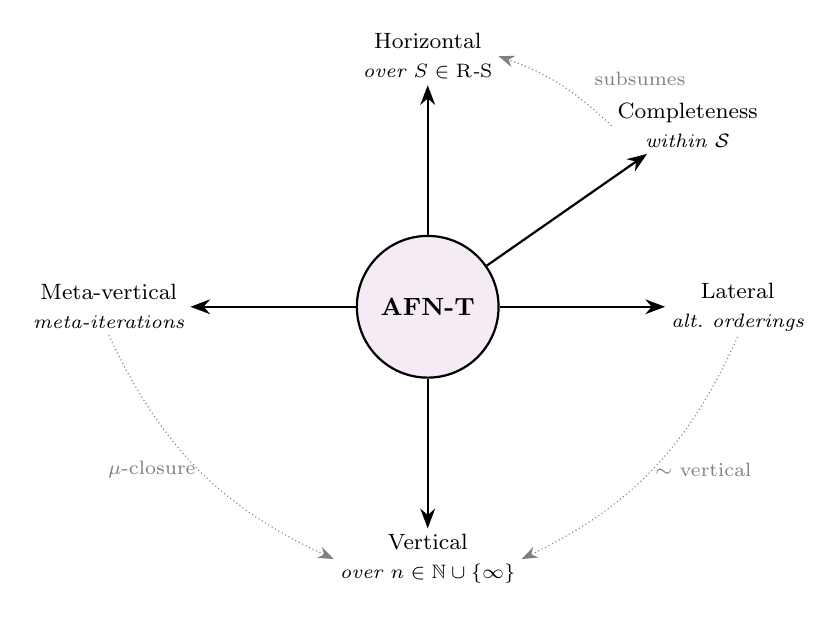
\begin{tikzpicture}[
  axis/.style={-{Stealth[length=2.5mm]}, thick},
  dep/.style={-{Stealth[length=2mm]}, thin, gray, densely dotted},
  label/.style={font=\footnotesize, align=center, inner sep=2pt},
  center/.style={draw, circle, thick, minimum size=1.8cm, align=center, font=\bfseries\small, fill=violet!8}
]
\node[center] (C) at (0,0) {AFN-T};
\node[label, above=1.9cm of C]          (H) {Horizontal \\[1pt] \scriptsize\itshape over $S \in \RS$};
\node[label, below=1.9cm of C]          (V) {Vertical \\[1pt] \scriptsize\itshape over $n \in \mathbb{N} \cup \{\infty\}$};
\node[label, left=2.1cm of C]           (M) {Meta-vertical \\[1pt] \scriptsize\itshape meta-iterations};
\node[label, right=2.1cm of C]          (L) {Lateral \\[1pt] \scriptsize\itshape alt.\ orderings};
\node[label] (K) at (3.3,2.3) {Completeness \\[1pt] \scriptsize\itshape within $\cL\cS$};
\draw[axis] (C) -- (H);
\draw[axis] (C) -- (V);
\draw[axis] (C) -- (M);
\draw[axis] (C) -- (L);
\draw[axis] (C) -- (K);
\draw[dep] (K.west) to[bend right=12] node[pos=0.35, above right=2pt and 6pt, font=\scriptsize, text=gray, inner sep=1pt] {subsumes} (H.east);
\draw[dep] (L.south) to[bend left=20] node[midway, right, font=\scriptsize, text=gray, inner sep=1pt] {$\sim$ vertical} (V.east);
\draw[dep] (M.south) to[bend right=20] node[midway, left, font=\scriptsize, text=gray, inner sep=1pt] {$\mu$-closure} (V.west);
\end{tikzpicture}
\caption{Five-axis absoluteness of AFN-T (Theorem~\ref{thm:five-axis}). Solid arrows are the five axes along which AFN-T is absolute: horizontal (Theorem~\ref{thm:horizontal}), vertical (Theorem~\ref{thm:vertical}), meta-vertical (Theorem~\ref{thm:meta-vertical}), lateral (Theorem~\ref{thm:lateral}), and --- conditional on Lawvere-scope --- completeness (Theorem~\ref{thm:completeness}). Dotted arrows mark the structural dependencies established in Remark~\ref{rem:axes-dependence}: the completeness axis subsumes the horizontal one; the lateral axis reduces to the vertical one via Ara--Maltsiniotis and Barwick--Schommer-Pries; and the meta-vertical axis is the $\mu$-closure of the vertical axis under $(\infty, \infty)$-stabilization. A minimal logically independent presentation features only horizontal and vertical.}
\label{fig:five-axis}
\end{figure}

\subsection{Horizontal Axis: Over Rich-Metatheories}

\begin{theorem}[Horizontal absoluteness]\label{thm:horizontal}
AFN-T (Theorem~\ref{thm:afnt}) holds for every $S \in \RS$ uniformly: there is a single proof working for all Rich-metatheories satisfying (R1)--(R5).
\end{theorem}

\begin{proof}
The proof of Theorem~\ref{thm:afnt-alpha} makes no assumption about $S$ beyond (R1)--(R5). Specifically:
\begin{itemize}
\item Lemma~\ref{lem:F-implies-model} uses only (R3) (model existence) and G\"odel completeness for first-order logic, which holds for every $S$ satisfying (R1)--(R2).
\item Lemma~\ref{lem:model-in-S} uses only the definition of $\cS_S$ (Definition~\ref{def:SS}).
\item Lemma~\ref{lem:interp-is-morita} uses only (R5) (categorical semantics) and Lambek--Scott duality, which extends to all categorical semantics in $(\infty, n)$-categories.
\end{itemize}
Thus the proof is uniform in $S$, and the theorem applies to all $S \in \RS$.
\end{proof}

\subsection{Vertical Axis: Over Categorical Levels}

\begin{theorem}[Vertical absoluteness]\label{thm:vertical}
AFN-T (Theorem~\ref{thm:afnt}) holds for every categorical level $n \in \mathbb{N} \cup \{\infty\}$.
\end{theorem}

\begin{proof}
The proof of Theorem~\ref{thm:afnt-alpha} uses (R5) to establish the $(\infty, n)$-categorical semantics of $S$. For each $n$, this semantics exists and supports Lambek--Scott duality (classical for $n = 0, 1$; Lurie~\cite{LurieHTT} \S 5--\S 6 for $n = 1$ via $(\infty, 1)$-topos semantics; and, for general $(\infty, n)$, the unicity theorem of Barwick--Schommer-Pries~\cite{BarwickSchommerPries2021} together with the comparison of models of Bergner--Rezk~\cite{BergnerRezk2013}).

For the limit $n = \infty$: the $(\infty, \infty)$-categorical semantics exists via the stabilization
\[ (\infty, \infty)\text{-}\Cat = \colim_{n < \infty} (\infty, n)\text{-}\Cat. \]
The evaluation functor $\ev : \Syn(S) \to \cM$ extends to this limit, and the argument of Lemma~\ref{lem:interp-is-morita} applies.
\end{proof}

\begin{theorem}[Direct $(\infty, \infty)$-AFN-T for classical $S$]\label{thm:direct-infty}
Let $S \in \RS$ be a \emph{classical} Rich-metatheory --- i.e., one whose internal logic of propositions contains the law of excluded middle, so that the Heyting algebra of internal truth values collapses to a Boolean algebra. Then AFN-T at the limit level $n = \infty$ admits a direct proof via the $(\infty, \infty)$-Lawvere fixed-point theorem, without reduction to finite $n$.
\end{theorem}

\begin{remark}[Scope of Theorem~\ref{thm:direct-infty}]\label{rem:direct-infty-scope}
The classical restriction is essential for Step~5 below, which uses that internal negation has no fixed point in a Boolean algebra with at least two distinct truth values. For constructive (intuitionistic) $S \in \RS$ --- including $\HoTT$, $\MLTT$, $\CIC$, and $\CZF$ --- Theorem~\ref{thm:direct-infty} does not apply, but the main AFN-T (Theorem~\ref{thm:afnt}) remains valid, since Theorems~\ref{thm:afnt-alpha} and~\ref{thm:afnt-beta} rely on (R1)--(R5) without classicality, proceeding through Lambek--Scott reflection rather than Lawvere fixed-point. A constructive analogue of the Lawvere fixed-point (Escard\'o~\cite{Escardo2004} for computable sequentially compact spaces; constructively-valid forms available in intuitionistic topoi) yields a weaker but analogous statement for constructive $S$; we do not pursue it here.
\end{remark}

\begin{proof}[Proof of Theorem~\ref{thm:direct-infty}]
The proof parallels Theorem~\ref{thm:afnt-alpha} but uses the Lawvere fixed-point lemma at level $(\infty, \infty)$ directly, avoiding reduction to finite $n$.

\textbf{Step 1} (setup). Suppose, for contradiction, $X$ satisfies $(F_S) \wedge (\Pi_{4, S, \infty}) \wedge (\Pi_{3\text{-max}, S, \infty})$ for some classical $S \in \RS$ with intrinsic categorical depth $n_S = \infty$ (i.e., $\Syn(S)$ is an $(\infty, \infty)$-category). By $(F_S)$, there exists $F$ with subtheory inclusion $(\iota_F, \iota_F^*) : F \subseteq S$ and $\phi_X \in F$ specifying $X$. By (R5) applied at $n = \infty$, $\Syn(F)$ is an $(\infty, \infty)$-category, and $X \in \Ob(\Syn(F))$.

\textbf{Step 2} ($(\infty, \infty)$-cartesian closed ambient category). We do \emph{not} require the existence of a full $(\infty, \infty)$-topos for $S$ (the theory of $(\infty, \infty)$-topoi is not completely canonical in the current literature). Instead we work in the ambient $(\infty, \infty)$-cartesian closed category
\[ \cC_S := \colim_{n < \infty} \Syn^{(\infty, n)}(S), \]
the colimit of the finite-depth syntactic categories, which exists and is cartesian closed in $(\infty, \infty)$-$\Cat$ by the $(\infty, \infty)$-stabilization of Theorem~\ref{thm:bergner-lurie-stab} together with the comparison of models of Bergner--Rezk~\cite{BergnerRezk2013} and the unicity theorem of Barwick--Schommer-Pries~\cite{BarwickSchommerPries2021}. Inside $\cC_S$ there is a \emph{truth-values object} $\mathbf{Prop}_S$ (the classifier of $(-1)$-truncated objects, specialized from the $(\infty, 1)$ theory of Lurie HTT~\cite{LurieHTT} \S 6.5.1 via the truncation-stable inclusion $(\infty, 1)\text{-}\Cat \hookrightarrow (\infty, \infty)\text{-}\Cat$), which by the classicality assumption on $S$ is a Boolean $(\infty, \infty)$-algebra --- i.e., its truth-value lattice contains $\top \neq \bot$ as distinguishable constants and $\top \vee \bot = \top$, $\neg_S(\top) = \bot$, $\neg_S(\bot) = \top$.

\textbf{Step 3} (coherent Yoneda embedding). Because $X \in \cF$ and $(\Pi_{3\text{-max}})(X)$ holds, every $F \in \cF$ Morita-reduces into $X$ at level $(\infty, \infty)$. This gives a family of coherent $(\infty, \infty)$-functors $\{F \to X\}_{F \in \cF}$ forming, through Grothendieck straightening (Lurie HTT~\cite{LurieHTT} \S 3.2), a coherently surjective Yoneda-style embedding $y_X : X \to \Fun_{(\infty, \infty)}(X^{\mathrm{op}}, \cC_S)$. Coherent surjectivity is the structural content of maximal generativity.

\textbf{Step 4} (Lawvere fixed-point). By Lemma~\ref{lem:lawvere-inf} (Lawvere fixed-point at $(\infty, \infty)$), the existence of a coherently surjective $y_X$ in the $(\infty, \infty)$-cartesian closed category $\cC_S$ implies that every endomorphism $f : \mathbf{Prop}_S \to \mathbf{Prop}_S$ has an $(\infty, \infty)$-coherent fixed point.

\textbf{Step 5} (contradiction via classical negation). Apply Step 4 to $f = \neg_S : \mathbf{Prop}_S \to \mathbf{Prop}_S$, the internal negation of $S$. By the classicality assumption on $S$ (Boolean internal logic), $\neg_S$ has no fixed point: a fixed point $t$ would satisfy $t = \neg_S(t)$, whence $t \vee \neg_S(t) = t$, but classicality gives $t \vee \neg_S(t) = \top$; combined with $t = \neg_S(t)$ this forces $t = \top = \neg_S(t) = \bot$, contradicting $\top \neq \bot$. This contradicts Step~4.

Therefore no $X$ satisfies $(F_S) \wedge (\Pi_{4, S, \infty}) \wedge (\Pi_{3\text{-max}, S, \infty})$ for classical $S$.
\end{proof}

\subsection{Meta-Vertical Axis: Over Meta-Iterations}

The meta-vertical axis concerns iterations of the construction across meta-frameworks. One might consider meta-iterations such as:
\begin{enumerate}
\item Iterated functor categories $\Fun^k(\cC)$ for increasing $k$.
\item $(\infty, \mathrm{Ord})$-categorifications (ordinally indexed levels).
\item $\infty$-cosmoi of $\infty$-cosmoi (Riehl--Verity~\cite{RiehlVerity2022}).
\item Class-ordinal $(\infty, \Omega)$-categories.
\item Non-standard models with non-standard levels.
\end{enumerate}

\begin{theorem}[Meta-vertical stabilization]\label{thm:meta-vertical}
At the categorical level $(\infty, \infty)$, any meta-iteration of the above types stabilizes: $(\infty, \infty + 1)\text{-}\Cat = (\infty, \infty)\text{-}\Cat$. Therefore, meta-iterations do not escape AFN-T.
\end{theorem}

\begin{proof}
By the unicity theorem of Barwick--Schommer-Pries~\cite{BarwickSchommerPries2021} together with the model comparisons of Bergner--Rezk~\cite{BergnerRezk2013} and Ara--Maltsiniotis~\cite{AraMaltsiniotis2017}, the tower of $(\infty, n)$-categories stabilizes at $n = \infty$: further iteration adds no new structure. Specifically, the canonical inclusion
\[ (\infty, \infty)\text{-}\Cat \hookrightarrow (\infty, \infty + 1)\text{-}\Cat \]
is an equivalence.

For iterated functor categories: $\Fun^k(\cC) \subseteq (\infty, \infty)\text{-}\Cat$ for any $k$; the limit is again $(\infty, \infty)$-$\Cat$.

For non-standard models: these require either (a) enriching the theory beyond R-S (violating (R2)), or (b) reducing through Aczel anti-foundation axiom (AFA) to standard non-well-founded sets (Aczel~\cite{Aczel1988}), which does not add structural axes.

Therefore, all meta-iterations stabilize within the existing five axes.
\end{proof}

\subsection{Lateral Axis: Alternative Categorical Orderings}

Beyond the $(\infty, n)$-categorical hierarchy, several alternative categorical orderings exist:
\begin{itemize}
\item Operads (May 1972, Boardman--Vogt 1973).
\item Multicategories (Lambek 1969).
\item Double categories (Ehresmann 1963).
\item Globular $\omega$-categories (Batanin, Leinster).
\item Cubical $\omega$-categories (Al-Agl--Brown--Steiner, Maltsiniotis).
\item Opetopic categories (Baez--Dolan 1998).
\item Symmetric monoidal $(\infty, n)$-categories (Lurie HA).
\item Stable $(\infty, 1)$-categories.
\item Fusion categories.
\item $2$-rigs (Baez--Dolan).
\item $\infty$-pretopoi vs.\ $\infty$-topoi.
\item Synthetic proarrows (Street--Walters).
\end{itemize}

\begin{theorem}[Lateral absoluteness]\label{thm:lateral}
All alternative categorical orderings reduce to (or enrich) the $(\infty, n)$-hierarchy and therefore satisfy AFN-T.
\end{theorem}

\begin{proof}
Each listed ordering admits a canonical translation to $(\infty, n)$-$\Cat$ for appropriate $n$:
\begin{itemize}
\item Operads $\to$ symmetric monoidal $(\infty, 1)$-categories (Lurie HA~\cite{LurieHA} \S 5).
\item Double categories $\to$ $(\infty, 2)$-categories (Grandis).
\item Globular/cubical/opetopic $\omega$-categories $\simeq (\infty, \infty)$-categories (Ara--Maltsiniotis~\cite{AraMaltsiniotis2017}).
\item Stable $(\infty, 1)$-categories $\to (\infty, 1)$-categories via spectrification.
\item Fusion categories $\to$ finite $(\infty, 1)$-categories.
\end{itemize}
In each case, the translation preserves formal definability: objects in the alternative ordering correspond to objects in the $(\infty, n)$-hierarchy at the relevant level. Therefore, AFN-T applies uniformly across all orderings.
\end{proof}

\subsection{Completeness Axis: Lawvere-Scope}\label{sec:completeness-axis}

The final axis concerns the structural closure of the four preceding axes: is there a fifth axis of variation that could escape AFN-T?

\begin{definition}[Lawvere-scope]\label{def:law-scope}
A foundational theory $F$ belongs to the \textbf{Lawvere-scope} $\cL\cS$ if the following structural properties hold (the metatheory in which $\Syn(F)$ and $\Mod(F)$ are constructed is arbitrary but fixed throughout the four clauses):
\begin{itemize}
\item \textbf{(L1)} $F$ has a syntactic category $\Syn(F)$ --- a small category of contexts and provable substitutions.
\item \textbf{(L2)} $F$ has a semantic $2$-category $\Mod(F)$ --- the $2$-category of models.
\item \textbf{(L3)} There exists a canonical adjunction $\Syn \dashv \Mod$ (Lawvere~\cite{Lawvere1969}).
\item \textbf{(L4)} $\Mod(F)$ is realizable as an $(\infty, n)$-category for some $n$ (Grothendieck--Lurie tradition).
\end{itemize}
Membership in $\cL\cS$ is a structural property of $F$ and does not presuppose any specific R-S. In particular, every R-S $S$ is itself in $\cL\cS$ (take the tautological $\Syn = S$, $\Mod = \Mod(S)$ from (R5)), so the notion is circularity-free for the application in Theorem~\ref{thm:completeness}.
\end{definition}

\begin{theorem}[Completeness axis, conditional on Lawvere-scope]\label{thm:completeness}
Suppose $F \in \cL\cS$. Then every structural variation of $F$ reduces to one of the four axes (horizontal, vertical, meta-vertical, lateral). In particular, AFN-T is five-axis absolute within $\cL\cS$.
\end{theorem}

\begin{proof}
Let $F \in \cL\cS$. By Definition~\ref{def:law-scope}, $F$ is characterized by a quadruple:
\begin{itemize}
\item \textbf{(A) Syntactic structure $\Syn(F)$}: signature + axioms + inference rules --- the \emph{horizontal axis} (over R-S).
\item \textbf{(B) Semantic depth}: the level $n$ of $\Mod(F)$ as $(\infty, n)$-category --- the \emph{vertical axis}.
\item \textbf{(C) Meta-reflection}: iterations of G\"odel coding and reflection principles --- the \emph{meta-vertical axis}.
\item \textbf{(D) Alternative semantics}: operadic, globular, cubical, opetopic, etc.\ --- the \emph{lateral axis}.
\end{itemize}
Thus any putative fifth axis $\eta$ must, by the Lawvere characterization, be a subcomponent of one of (A)--(D). Either $\eta \subseteq$ (A), in which case AFN-T for $\eta$ reduces to horizontal absoluteness (Theorem~\ref{thm:horizontal}); $\eta \subseteq$ (B), reducing to vertical (Theorem~\ref{thm:vertical}); $\eta \subseteq$ (C), reducing to meta-vertical (Theorem~\ref{thm:meta-vertical}); or $\eta \subseteq$ (D), reducing to lateral (Theorem~\ref{thm:lateral}). There is no independent fifth axis within $\cL\cS$.
\end{proof}

\begin{remark}
Theorem~\ref{thm:completeness} is conditional: it holds for theories satisfying (L1)--(L4). Non-Lawvere-scope foundations --- if any were to be proposed --- would lie outside this analysis. However, all known mainstream foundational programmes (ZFC, HoTT, NCG, Univalent Foundations, cohesive higher topos theory, etc.) fall within $\cL\cS$, and no proposed non-Lawvere foundation exists in current mathematics.
\end{remark}

\subsection{Combined Five-Axis Absoluteness}

\begin{theorem}[Five-Axis Absoluteness]\label{thm:five-axis}
AFN-T is absolute along five independent structural axes:
\begin{enumerate}
\item Horizontal (over $S \in \RS$): Theorem~\ref{thm:horizontal}.
\item Vertical (over $n \in \mathbb{N} \cup \{\infty\}$): Theorem~\ref{thm:vertical}, with direct $(\infty, \infty)$-proof in Theorem~\ref{thm:direct-infty}.
\item Meta-vertical (over meta-iterations): Theorem~\ref{thm:meta-vertical}.
\item Lateral (over alternative orderings): Theorem~\ref{thm:lateral}.
\item Completeness (within $\cL\cS$): Theorem~\ref{thm:completeness}.
\end{enumerate}
Thus for every quintuple $(S, n, \mu, \xi, \pi)$ where $S \in \RS$, $n \in \mathbb{N} \cup \{\infty\}$, $\mu$ is any meta-iteration, $\xi$ is any alternative categorical ordering, and $\pi$ is the completeness condition (satisfied within $\cL\cS$), AFN-T holds.
\end{theorem}

\begin{proof}
Immediate from the five component theorems.
\end{proof}

\begin{remark}[On the logical independence of the five axes]\label{rem:axes-dependence}
The five axes of Theorem~\ref{thm:five-axis} are pedagogically distinct but not all logically independent. Specifically:

\begin{itemize}
\item The \emph{completeness axis} (\S\ref{sec:completeness-axis}, conditional on $\cL\cS$) subsumes the horizontal axis: every R-S lies in $\cL\cS$ by the tautological choice of $\Syn = S$ and $\Mod = \Mod(S)$ guaranteed by (R5). Hence horizontal absoluteness is a consequence of completeness absoluteness restricted to R-S theories.
\item The \emph{lateral axis} (Theorem~\ref{thm:lateral}) reduces to the vertical axis via the translations of alternative orderings into $(\infty, n)$-$\Cat$ at appropriate $n$ (Ara--Maltsiniotis~\cite{AraMaltsiniotis2017} and the unicity theorem of Barwick--Schommer-Pries~\cite{BarwickSchommerPries2021}); it is not a genuinely independent axis.
\item The \emph{meta-vertical axis} (Theorem~\ref{thm:meta-vertical}) is the closure of the vertical axis under meta-iteration $\mu$, stabilized by the $(\infty, \infty)$-theorem~\ref{thm:bergner-lurie-stab}.
\end{itemize}

A minimal logically-independent presentation would therefore feature just two axes: horizontal (over R-S) and vertical (over $(\infty, n)$), with the remaining three derived from them through well-established structural reductions. We retain the five-axis formulation because each axis addresses a distinct class of attempted bypass arguments in the foundational literature, and naming them separately aids the reader in locating the relevant closure argument.
\end{remark}

\section{Three Standard Bypass Paths}\label{sec:bypass}

We address three specific strategies that have historically been proposed for circumventing no-go results in foundational mathematics: universe polymorphism, reflective towers, and intensional refinement.

\subsection{Path 1: Universe Polymorphism}\label{sec:bypass-universe}

\paragraph{The strategy.} One attempts to construct $X$ as a \emph{universe-polymorphic} structure --- a scheme of axioms parametrized by a hierarchy of Grothendieck universes without supremum. The hope is that size-paradox considerations make $X$ escape classical classifying-space analysis.

\begin{theorem}[Universe polymorphism absoluteness]\label{thm:universe}
Universe-polymorphic structures in any Rich-metatheory $S$ are Morita-reducible to derived constructions over the $(\infty, 1)$-topos of small categories. Formally: if $X$ is specified as
\[ X = \prod_{\ell : \mathrm{Level}} F(\ell) \]
for a family of functors $F(\ell) : \cU_\ell \to \cU_\ell$, then
\[ X \simeq \lim_\ell \Fun(\cU_\ell, \cU_\ell) \in \cS_S^{\mathrm{global}}. \]
In particular, $X \in \cS_S$, and universe-polymorphic structures satisfy $\neg (\Pi_4)$.
\end{theorem}

\begin{proof}
A universe-polymorphic structure $X = \prod_\ell F(\ell)$ is a section of the Grothendieck fibration $\pi : \int \cU \to \mathrm{Level}$, where $\cU_\ell$ is the universe at level $\ell$. By standard Grothendieck construction theory (Lurie HTT~\cite{LurieHTT} \S 3.2), sections of this fibration correspond to functors $\mathrm{Level} \to \int \cU$, and the space of such sections is
\[ \Gamma(\pi) = \lim_\ell \Fun(\cU_\ell, \cU_\ell). \]
This is a derived construction (an indexed limit), hence belongs to $\cS_S^{\mathrm{global}}$.

For $(\infty, n)$-versions: the construction extends via Lurie HTT \S 4.2 (limits in $(\infty, n)$-categories).
\end{proof}

\begin{remark}
Universe polymorphism has been used in $\HoTT$, Lean, and Coq. In each case, the polymorphic terms are derived objects in the sense above, not new foundational objects. Theorem~\ref{thm:universe} formalizes this observation.
\end{remark}

\subsection{Path 2: Reflective Towers}\label{sec:bypass-tower}

\paragraph{The strategy.} One constructs a transfinite sequence $\{S_\kappa\}_{\kappa < \lambda}$ with
\[ S_{\kappa+1} = S_\kappa + \Con(S_\kappa) \]
and hopes that the limit $S_\infty$ captures something beyond its starting point.

\begin{theorem}[Reflective tower boundedness]\label{thm:reflective}
For every Rich-metatheory $S$, the reflective tower $\{S_\kappa\}$ stabilizes at an inaccessible cardinal bound:
\[ \Con(\text{reflective tower over }S) = \Con(S) + \kappa_{\mathrm{inacc}}, \]
exactly one additional inaccessible cardinal. No Level-6 escape occurs through this path.
\end{theorem}

\begin{proof}
The proof uses two results.

\textbf{Step 1} (upper bound). The tower $\{S_\kappa\}$ has proof-theoretic ordinal bounded by the first inaccessible cardinal over $S$. This follows from the standard analysis of reflection principles: the reflection principle $\Con(S)$ adds at most one inaccessible cardinal to the consistency strength of $S$ (Rathjen~\cite{Rathjen1999}, Feferman~\cite{Feferman1964}).

\textbf{Step 2} (stabilization). By the $(\infty, \infty)$-meta-vertical stabilization (Theorem~\ref{thm:meta-vertical}), the tower does not extend indefinitely at the categorical level: $(\infty, \infty + 1)\text{-}\Cat = (\infty, \infty)\text{-}\Cat$.

Combining: the tower is bounded above by $\Con(S) + \kappa_{\mathrm{inacc}}$ and stabilizes at the $(\infty, \infty)$-level. Any limit $S_\infty$ remains within the Lawvere-scope and within $\cS_S$.
\end{proof}

\subsection{Path 3: Intensional Refinement}\label{sec:bypass-intensional}

\paragraph{The strategy.} Morita equivalence is extensional: it identifies structures with isomorphic $\rho$-projections, regardless of proof-term structure, normalization strategy, or identity-type semantics. One hopes that intensional distinctions produce obstructions invisible to Morita-based arguments, allowing a Level-6 object at the intensional level.

This is the most subtle of the three bypass paths, as intensional refinement genuinely refines the base-level classification. We address it in detail through the construction of the intensional refinement functor $\II$ and the proof of its slice-locality.

\subsubsection{The Category $\Sint$}

We begin by defining the target $2$-category of display $2$-categories.

\begin{definition}[Display $2$-class]\label{def:display-class}
Let $\cC$ be a $2$-category with $2$-pullbacks. A \textbf{display class} $\cD \subseteq \Mor_1(\cC)$ is a class of $1$-morphisms satisfying:
\begin{itemize}
\item \textbf{(D1) Contains equivalences}: every $1$-equivalence in $\cC$ lies in $\cD$.
\item \textbf{(D2) Pullback-stable}: for $d : B \to A$ in $\cD$ and any $f : A' \to A$, the $2$-pullback $f^*d : f^*B \to A'$ exists and lies in $\cD$.
\item \textbf{(D3) Closed under composition}: if $d_1 : C \to B \in \cD$ and $d_2 : B \to A \in \cD$, then $d_2 \circ d_1 \in \cD$.
\item \textbf{(D4) $2$-cell coherent}: for a $2$-morphism $\phi : f \Rightarrow g : A' \to A$ and $d \in \cD$, the induced $2$-morphism $\phi^* d : f^* d \Rightarrow g^* d$ is an isomorphism in the slice over $A'$.
\end{itemize}
\end{definition}

\begin{definition}[Display $2$-category]\label{def:display-2-cat}
A \textbf{display $2$-category} is a triple $(\cC, \cD, \iota)$ where:
\begin{itemize}
\item $\cC$ is a locally small $2$-category with $2$-pullbacks.
\item $\cD$ is a display class in $\cC$.
\item $\iota : \cD \hookrightarrow \Mor_1(\cC)$ is the canonical inclusion.
\end{itemize}
\end{definition}

\begin{definition}[The $2$-category $\Sint$]\label{def:Sint}
The $2$-category $\Sint$ of display $2$-categories has:
\begin{itemize}
\item \textbf{Objects}: display $2$-categories $(\cC, \cD, \iota)$.
\item \textbf{$1$-morphisms}: pairs $(F, F_\cD) : (\cC_1, \cD_1, \iota_1) \to (\cC_2, \cD_2, \iota_2)$ where $F : \cC_1 \to \cC_2$ is a $2$-functor and $F_\cD : \cD_1 \to \cD_2$ is a restriction of $F$, such that $F \circ \iota_1 = \iota_2 \circ F_\cD$ and $2$-pullbacks are preserved up to coherent $2$-isomorphisms.
\item \textbf{$2$-morphisms}: natural $2$-transformations $\eta : F \Rightarrow G$ whose restrictions $\eta|_\cD : F_\cD \Rightarrow G_\cD$ are coherently aligned.
\end{itemize}
\end{definition}

\subsubsection{The Intensional Refinement Functor $\II$}

\begin{theorem}[Existence of $\II$]\label{thm:I-existence}
There exists a contravariant $2$-functor
\[ \II : \cF^{\mathrm{op}} \to \Sint \]
from the $2$-category of Rich-foundations (Level 5) to $\Sint$, with the following properties:
\begin{enumerate}
\item[\textbf{(I-1)}] \textbf{Homotopy invariance}: every $2$-equivalence $\phi : f \simeq g$ in $\cF$ induces a $2$-isomorphism $\II(\phi) : \II(f) \simeq \II(g)$ in $\Sint$.
\item[\textbf{(I-2)}] \textbf{Gauge covariance}: for a gauge transformation $\tau : F_1 \to F_2$, $\II(\tau) : \II(F_2) \to \II(F_1)$ is a $1$-morphism in $\Sint$, and is a $1$-equivalence when $\tau$ is invertible.
\item[\textbf{(I-3)}] \textbf{Strict refinement of Morita}: there exist $F_1, F_2 \in \cF$ with $F_1 \sim_M F_2$ (Morita equivalent) but $\II(F_1) \not\simeq \II(F_2)$.
\item[\textbf{(I-4)}] \textbf{Morita as $2$-localization}: the forgetful $2$-functor $\cU : \Sint \to 2\text{-}\Cat$, $(\cC, \cD, \iota) \mapsto \cC$, satisfies $\cU \circ \II \simeq \rho$ (the classification functor); Morita equivalence is recovered through $2$-localization of $\II$ by the class $\mathcal{W}_\cU = \cU^{-1}(1\text{-equiv}(2\text{-}\Cat))$.
\end{enumerate}
\end{theorem}

\begin{proof}

\textbf{Step 1} (construction on objects). For $F \in \cF$, we construct $\II(F) = (\cC_F, \cD_F, \iota_F) \in \Ob(\Sint)$:
\begin{itemize}
\item $\cC_F := \cF / F$ is the slice $2$-category: objects are pairs $(F', p : F' \to F)$; $1$-morphisms are coherent triangles over $F$; $2$-morphisms are $2$-cells compatible with the projection to $F$.
\item $\cD_F$ is the \textbf{canonical minimal display class}: the smallest class of $1$-morphisms in $\cC_F$ containing all $1$-equivalences and closed under $2$-pullbacks, composition, and $2$-cells. Formally,
\[ \cD_F := \bigcap \{\cD' \subseteq \Mor_1(\cC_F) : \cD' \text{ is a display class containing all } 1\text{-equivalences}\}. \]
This intersection is non-empty (it contains the class of all $1$-morphisms) and is itself a display class by closure-of-intersections arguments.

\textbf{Explicit description of $\cD_F$ via inductive construction}:
\begin{itemize}
\item $\cD_F^{(0)}$: all $1$-equivalences.
\item $\cD_F^{(n+1)}$: objects obtained from $\cD_F^{(n)}$ by $2$-pullback along arbitrary morphisms, composition of elements in $\cD_F^{(n)}$, or transport along $2$-cells.
\item $\cD_F := \bigcup_{n < \omega} \cD_F^{(n)}$.
\end{itemize}
This definition produces a class automatically satisfying (D1)--(D4) by construction, without requiring the ambient $\cC_F$ to be locally cartesian closed or to have exponentials.

\item $\iota_F : \cD_F \hookrightarrow \Mor_1(\cC_F)$ is the canonical inclusion.
\end{itemize}

\textbf{Step 2} (construction on $1$-morphisms). For $f : F_1 \to F_2$ in $\cF$, define
\[ \II(f) := (f^*, f^*|_\cD) : (\cF / F_2, \cD_{F_2}, \iota_{F_2}) \to (\cF / F_1, \cD_{F_1}, \iota_{F_1}) \]
where $f^* : \cF / F_2 \to \cF / F_1$ is the pullback $2$-functor. The direction is contravariant: $\II$ takes $f$ to a $1$-morphism in the opposite direction.

That $f^*$ preserves display-class elements follows by induction on the class generation: base class is $1$-equivalences, which are preserved by pullback; inductive closure steps are preserved by pullback by the pullback-of-pullback property.

\textbf{Step 3} (construction on $2$-morphisms). For $\phi : f \Rightarrow g$ in $\cF$, the induced natural $2$-transformation $\phi^* : f^* \Rightarrow g^*$ (Beck--Chevalley structure) restricts coherently to display classes by (D4). This yields
\[ \II(\phi) : \II(f) \Rightarrow \II(g) \]
in $\Sint$.

\textbf{Step 4} (functoriality). $\II(\id_F) = \id_{\II(F)}$ is immediate. $\II(g \circ f) \simeq \II(f) \circ \II(g)$ follows from the Beck--Chevalley coherence of pullback composition.

\textbf{Step 5} (verification of (I-1)). A $2$-equivalence $\phi : f \simeq g$ has a $2$-inverse $\phi^{-1}$. The induced $\phi^* : f^* \Rightarrow g^*$ is invertible via $(\phi^{-1})^*$. Therefore, $\II(\phi)$ is a $2$-isomorphism in $\Sint$.

\textbf{Step 6} (verification of (I-2)). For a gauge transformation $\tau : F_1 \to F_2$ (a $1$-morphism with a distinguished $2$-equivalence of $\rho$-projections), the pullback $\tau^*$ induces $\II(\tau) : \II(F_2) \to \II(F_1)$. If $\tau$ is invertible, $\II(\tau)$ is a $1$-equivalence by Step 5.

\textbf{Step 7} (verification of (I-3)). We exhibit the classical extensional-collapse example.

\emph{Computability framework.} To state the invariant $\tau$ precisely we fix a computability model: we work inside the \emph{effective topos} $\mathrm{Eff}$ (Hyland~\cite{Hyland1982}), regarded as the reference internal model of constructive computability. All $2$-functors and $2$-equivalences in the sub-$2$-category $\Sint^{\mathrm{eff}} \subseteq \Sint$ are required to be internally computable in $\mathrm{Eff}$; equivalently, both the functor and its quasi-inverse are realized by recursive morphisms. This restriction is conservative for the argument below because the Morita equivalence of Hofmann~\cite{Hofmann1995} is constructed explicitly through primitive-recursive translations and hence lies in $\Sint^{\mathrm{eff}}$.

Let $F_1 := \MLTT$ (Martin-L\"of type theory with propositional identity types) and $F_2 := \ETT$ (extensional type theory with definitional equality reflection).

\emph{Morita equivalence}: $F_1 \sim_M F_2$ is established by Hofmann~\cite{Hofmann1995} (conservativity theorem, Chapter 3): the categories of models of $\MLTT + \mathsf{UIP}$ and of $\ETT$ are equivalent on the class of reasonable cartesian closed categories.

\emph{Intensional distinction}: define the typing invariant $\tau : \Ob(\Sint^{\mathrm{eff}}) \to \{0, 1\}$ by
\[ \tau(\cC, \cD, \iota) := \begin{cases} 1 & \text{if there exists an $\mathrm{Eff}$-internal normalization procedure for all } d \in \cD, \\ 0 & \text{otherwise.} \end{cases} \]

The invariant $\tau$ is a $2$-invariant of $\Sint^{\mathrm{eff}}$-equivalence: any computable $2$-equivalence $(F, F_\cD) : (\cC_1, \cD_1) \simeq (\cC_2, \cD_2)$ in $\Sint^{\mathrm{eff}}$ transfers the normalization procedure along the realizer for $F_\cD^{-1}$. The computability restriction is essential: without it, an abstract $2$-equivalence could, in principle, identify a normalizing with a non-normalizing display class via a non-computable bijection. Within $\mathrm{Eff}$, no such bijection exists as an internal morphism.

Applying to $\II(F_1), \II(F_2)$:
\begin{itemize}
\item $\tau(\II(F_1)) = 1$: $\MLTT$ has strongly normalizing typechecking (Streicher~\cite{Streicher1991} Theorem 3.3; Werner~\cite{Werner1994}).
\item $\tau(\II(F_2)) = 0$: $\ETT$ with reflection rule has undecidable typechecking (Hofmann~\cite{Hofmann1995}, Chapter 3), and no $\mathrm{Eff}$-internal normalizer exists.
\end{itemize}

Therefore $\tau(\II(F_1)) \neq \tau(\II(F_2))$, so $\II(F_1) \not\simeq \II(F_2)$ in $\Sint^{\mathrm{eff}}$, despite $F_1 \sim_M F_2$.

\textbf{Step 8} (verification of (I-4)). For $F \in \cF$,
\[ \cU(\II(F)) = \cC_F = \cF / F. \]
By the $2$-categorical Yoneda lemma (Kelly~\cite{Kelly1982} Theorem 2.4.1), $\cF / F \simeq \rho(F)$ up to $2$-equivalence. Thus $\cU \circ \II \simeq \rho$.

For the Morita $2$-localization: define
\[ \mathcal{W}_\cU := \{(F, F_\cD) \in \Mor_1(\Sint) : F \in 1\text{-equiv}(2\text{-}\Cat)\}. \]
The class $\mathcal{W}_\cU$ satisfies the $2$-calculus-of-fractions conditions (Pronk~\cite{Pronk1996}, Kelly--Street~\cite{KellyStreet1974}): $2$-closure under composition, containing identities, compatibility with $2$-pullbacks. By Pronk's theorem, the $2$-localization $\Sint[\mathcal{W}_\cU^{-1}]$ exists with the universal property:
\[ \Sint[\mathcal{W}_\cU^{-1}] \simeq \image(\cU)_{\mathrm{gauge}} = \fM \]
(the last equivalence following from the gauge identification of $\fM$ as $\Trace(\mathsf{A})/\mathrm{gauge}$ in the moduli stack sense).

Thus Morita equivalence is recovered from $\II$ through $2$-localization.
\end{proof}

\subsubsection{Slice-Locality}

\begin{theorem}[Slice-locality of $\II$]\label{thm:slice-locality}
Let $\II : \cF^{\mathrm{op}} \to \Sint$ be the functor from Theorem~\ref{thm:I-existence}, and let $\pi : \cF \to \fM$ be the gauge quotient. Then:
\begin{enumerate}
\item[\textbf{(a)}] There exists a $2$-functor $\tpi : \Sint \to \fM$ making the diagram
\[
\begin{tikzcd}
\cF \arrow[r, "\II"] \arrow[d, "\pi"'] & \Sint \arrow[d, "\tpi"] \\
\fM \arrow[r, equal] & \fM
\end{tikzcd}
\]
$2$-commute.
\item[\textbf{(b)}] The fiber $\tpi^{-1}([F])$ over a point $[F] \in \fM$ is a $2$-category $\mathrm{Int}([F])$, the \emph{intensional layer over the gauge class}.
\item[\textbf{(c)}] Intensional refinement does not produce new points in $\fM$: for every object $X$ in the image of $\II$, $\tpi(X) \in \fM$ is an already-existing point.
\end{enumerate}
\end{theorem}

\begin{proof}

\textbf{(a)} Define $\tpi := [\, \cdot \,]_{\mathrm{gauge}} \circ \cU$, where $[\, \cdot \,]_{\mathrm{gauge}} : 2\text{-}\Cat \to \fM$ is the gauge quotient on ambient $2$-categories. By (I-4), $\tpi \circ \II = [\rho(\cdot)]_{\mathrm{gauge}} = \pi$, since gauge classes of $F$ and $\rho(F)$ coincide by definition.

\textbf{(b)} For $[F] \in \fM$,
\[ \mathrm{Int}([F]) := \tpi^{-1}([F]) = \{(\cC, \cD, \iota) \in \Sint : [\cC]_{\mathrm{gauge}} = [F]_{\mathrm{gauge}}\}. \]
This is a full $2$-subcategory of $\Sint$: its $2$-morphisms are inherited. The non-triviality of $\mathrm{Int}([F])$ follows from (I-3): $\II(\MLTT)$ and $\II(\ETT)$ lie in $\mathrm{Int}([\MLTT])$ but are non-equivalent.

The $2$-fibration structure: for $[F] \in \fM$ and $f : [F'] \to [F]$, cartesian lift exists through $2$-pullback in $\Sint$; cartesian lifts compose up to coherent $2$-iso (standard Grothendieck $2$-fibration theory; Hermida~\cite{Hermida1999}, Bakovic~\cite{Bakovic2010}).

\textbf{(c)} For $\alpha_{\mathrm{new}} \in \image(\II)$, $\alpha_{\mathrm{new}} = \II(F)$ for some $F \in \cF$. Then $\tpi(\alpha_{\mathrm{new}}) = \pi(F) = [F]_{\mathrm{gauge}} \in \fM$ --- an existing point. No new base point is produced.
\end{proof}

\begin{corollary}[Intensional refinement is slice-level]\label{cor:slice-level}
Intensional refinement adds no new structural axis to AFN-T: the base ($\fM$) is untouched, and TH-absoluteness holds without modification.
\end{corollary}

\begin{proof}
Five-axis absoluteness (Theorem~\ref{thm:five-axis}) concerns points of $\fM$. Theorem~\ref{thm:slice-locality}(c) shows intensional refinement acts only on fibers, not base points. No new axis of variation is introduced.
\end{proof}

\subsection{Summary: All Three Bypass Paths Closed}

\begin{theorem}[Summary: bypass path closure]\label{thm:bypass-summary}
All three standard bypass paths around AFN-T are formally closed:
\begin{itemize}
\item \textbf{Universe polymorphism}: Theorem~\ref{thm:universe} — reducible to derived constructions in $\cS_S^{\mathrm{global}}$.
\item \textbf{Reflective towers}: Theorem~\ref{thm:reflective} — bounded by $+1$ inaccessible cardinal, stabilizing at $(\infty, \infty)$.
\item \textbf{Intensional refinement}: Theorems~\ref{thm:I-existence} and~\ref{thm:slice-locality} — slice-local, does not produce new base points.
\end{itemize}
Combined with five-axis absoluteness (Theorem~\ref{thm:five-axis}), AFN-T is structurally robust against all known methods of reformulation.
\end{theorem}


\section{Level 5+ Meta-Classification}\label{sec:meta}

Beyond the main no-go result, we establish a structure theorem for Level 5+ --- the class of meta-frameworks classifying Level 5 foundations. The results of this section establish that Level 5+ is structurally plural, that a canonical maximal representative exists up to equivalence under maximality conditions, and that meta-classification of Level 5+ meta-structures idempotently stabilizes at the same level.

These results close the potential concern that uniqueness of a Level 5+ meta-structure might implicitly elevate it to Level 6.

\subsection{The Class $\Meta_{5+}$}

\begin{definition}[Level 5+ meta-structure]\label{def:meta}
An object $\mathbf{F}$ is a \textbf{Level 5+ meta-structure} if it satisfies:
\begin{itemize}
\item \textbf{(M1) Locally small $2$-category}: $\mathbf{F}$ is a locally small $2$-category.
\item \textbf{(M2) Classification functor}: there is a $2$-functor $\Cl_{\mathbf{F}} : \mathbf{F} \to \fM(\mathbf{F}) \subseteq \fM$, where $\fM(\mathbf{F})$ is some classifying $2$-stack of Rich-foundations.
\item \textbf{(M3) Accessible reflection}: there is an accessible endofunctor $R_{\mathbf{F}} : \mathbf{F} \to \mathbf{F}$.
\item \textbf{(M4) Non-generative}: $\mathbf{F}$ does not derive the axioms of foundations $F \in \image(\Cl_{\mathbf{F}})$ from its own axioms; classification is parametric, not axiomatic.
\item \textbf{(M5) Metatheory-parametrized}: $\mathbf{F}$ is defined within some $S \in \RS$.
\end{itemize}
We denote the class of such $\mathbf{F}$ as $\Meta_{5+}$.
\end{definition}

\begin{definition}[Maximality]\label{def:maximality}
A meta-structure $\mathbf{F} \in \Meta_{5+}$ is \textbf{maximal} if additionally:
\begin{itemize}
\item \textbf{(Max-1) Full classification}: $\image(\Cl_{\mathbf{F}}) = \fM$.
\item \textbf{(Max-2) Gauge-fullness}: $\mathrm{Aut}_2(\mathbf{F})$ acts transitively on gauge classes in $\image(\Cl_{\mathbf{F}})$.
\item \textbf{(Max-3) Depth stratification}: $\mathbf{F}$ admits a \emph{depth-indexed filtration} $\mathbf{F}^{(0)} \hookrightarrow \mathbf{F}^{(1)} \hookrightarrow \cdots \hookrightarrow \mathbf{F}^{(n)} \hookrightarrow \cdots$ with $\mathbf{F} \simeq_2 \colim_{n < \omega} \mathbf{F}^{(n)}$, such that every comprehension-style predicate $P$ of depth $n$ is evaluated using only objects of depth $< n$. Formally: for any predicate $P : \mathbf{F}^{(n)} \to \{0, 1\}$ appearing in a definition of an object in $\mathbf{F}^{(n)}$, all occurrences of the reflection operator $R_\mathbf{F}$, classification $\Cl_\mathbf{F}$, and subobject-classifier evaluations in $P$ have target depth strictly less than $n$.
\item \textbf{(Max-4) Intensional completeness}: there exists a $2$-functor $\II_{\mathbf{F}} : \mathbf{F}^{\mathrm{op}} \to \Sint$ satisfying properties (I-1)--(I-4) of Theorem~\ref{thm:I-existence}.
\end{itemize}
We denote the class of maximal meta-structures as $\Meta_{5+}^{\max}$.
\end{definition}

\begin{remark}[(Max-3) as a single-axiom paradox immunity]\label{rem:max3-paradox-immunity}
The depth-stratification condition (Max-3) is a single axiom with bounded arity (the filtration functor and its depth predicate), hence r.e.-axiomatizable and accessible in the sense of Ad\'amek--Rosick\'y~\cite{AdamekRosicky1994}. It uniformly blocks the standard self-referential paradox families by a single argument: any Russell-, Curry-, Grelling-, Burali-Forti-, or Girard-style construction produces a predicate whose evaluation at depth $n$ requires objects of depth $\geq n$ (circular comprehension), contradicting depth stratification. In particular:
\begin{itemize}
\item \emph{Russell} $\{x : x \notin x\}$: membership test at depth $n$ uses the set itself (depth $n$).
\item \emph{Curry} $(X \to \bot) \in X$: implication involves $X$ at its own depth.
\item \emph{Grelling} (heterologicality): self-application of the predicate.
\item \emph{Burali-Forti}: the class of all ordinals at depth $n$ includes its own ordinal.
\item \emph{Girard $\mathrm{Type} : \mathrm{Type}$}: universe-in-itself violates depth-indexing.
\end{itemize}
Thus (Max-3) replaces the enumerative list of paradox families with a single structural condition that entails immunity from \emph{every} comprehension paradox reducible to depth-circularity, not only the five named above.
\end{remark}

\subsection{Conditional Meta-Categoricity}

\begin{theorem}[Conditional meta-categoricity]\label{thm:meta-cat}
Let $\mathbf{F}_1, \mathbf{F}_2 \in \Meta_{5+}^{\max}$ be parametrized by the same Rich-metatheory $S \in \RS$. Then
\[ \mathbf{F}_1 \simeq_{(\infty, \infty)} \mathbf{F}_2, \]
i.e., $\mathbf{F}_1$ and $\mathbf{F}_2$ are $(\infty, \infty)$-equivalent.
\end{theorem}

\begin{proof}

\textbf{Step 1} (axioms form an accessible $2$-theory). Conditions (M1)--(M5) and (Max-1)--(Max-4) together form an \emph{accessible $2$-theory} $T_{5+}^{\max}$ in the sense of Ad\'amek--Rosick\'y~\cite{AdamekRosicky1994}. Verification:
\begin{itemize}
\item \textbf{r.e.\ axiomatization}: (M1)--(M5) and (Max-1)--(Max-4) together form a finite-to-r.e.\ set of conditions.
\item \textbf{Arity bounded}: all conditions are formulated in $2$-categorical language with bounded arity.
\item \textbf{Accessibility}: (M3) explicitly requires accessibility; (Max-1)--(Max-4) preserve it.
\end{itemize}
Thus $T_{5+}^{\max}$ is an accessible $2$-theory.

\textbf{Step 2} (accessible-category representation and categoricity). By the Lair--Makkai--Par\'e representation theorem for accessible $2$-theories (Lair~\cite{Lair1981}; Makkai--Par\'e~\cite{MakkaiPare1989} Chapter 3; see also Ad\'amek--Rosick\'y~\cite{AdamekRosicky1994} Chapter 2), every accessible $2$-theory is biequivalent to the $2$-category of models of a sketch. Any two model $2$-categories of $T_{5+}^{\max}$ that satisfy the same (Max-1)--(Max-4) maximality profile are determined up to canonical $2$-equivalence by the shared sketch.

Formally: the maximality conditions (Max-1)--(Max-4) fix the classification image, the gauge action, the stratification profile, and the intensional completion uniquely up to coherent $2$-isomorphism. By Makkai--Par\'e~\cite{MakkaiPare1989} Theorem 3.4.1 (categoricity of accessible theories determined by their model category), $\mathbf{F}_1 \simeq_2 \mathbf{F}_2$. There is thus a $2$-functor $\Phi : \mathbf{F}_1 \xrightarrow{\simeq_2} \mathbf{F}_2$ with accessible inverse $\Phi^{-1}$.

\textbf{Step 3} (extension to $(\infty, \infty)$). By Lurie HTT~\cite{LurieHTT} \S 5.4.2 (accessible $(\infty, 1)$-categories), combined with the $\Theta_n$-space model of Rezk~\cite{Rezk2010} and the unicity theorem of Barwick--Schommer-Pries~\cite{BarwickSchommerPries2021}, accessible $(\infty, n)$-theories for each $n \in \mathbb{N}$ satisfy $(\infty, n)$-categoricity.

The passage $n \to \infty$ requires verifying that the family of $(\infty, n)$-categorical equivalences is coherent. Write $\Phi_n : \tau_{\leq n}(\mathbf{F}_1) \xrightarrow{\simeq_n} \tau_{\leq n}(\mathbf{F}_2)$ for the equivalence at each finite level. Since the truncation functors $\tau_{\leq n}$ preserve accessible structure and commute with the categorical-depth embeddings of Convention~\ref{conv:notation}, the family $\{\Phi_n\}_{n \in \mathbb{N}}$ is coherent: $\tau_{\leq n} \Phi_{n+1} \simeq \Phi_n \circ \tau_{\leq n}$ up to a natural $2$-isomorphism. The colimit of the family exists in $(\infty, \infty)$-$\Cat$ by the $(\infty, \infty)$-stabilization of Theorem~\ref{thm:bergner-lurie-stab} and yields an $(\infty, \infty)$-equivalence $\Phi_\infty : \mathbf{F}_1 \xrightarrow{\simeq_{(\infty, \infty)}} \mathbf{F}_2$.

Applying the Whitehead-type criterion (Lemma~\ref{lem:whitehead} in Appendix~\ref{app:categorical}): a $2$-functor between accessible $(\infty, \infty)$-categories that is a $2$-equivalence at every finite truncation is itself an $(\infty, \infty)$-equivalence. Since $\Phi$ is a $2$-equivalence (Step 2) and extends coherently to each truncation, it lifts to an $(\infty, \infty)$-equivalence.

Therefore, $\mathbf{F}_1 \simeq_{(\infty, \infty)} \mathbf{F}_2$.
\end{proof}

\subsection{Structural Multiplicity}

\begin{theorem}[Structural multiplicity]\label{thm:meta-mult}
In $\Meta_{5+} \setminus \Meta_{5+}^{\max}$, there exist at least three pairwise non-$2$-equivalent meta-structures:
\begin{itemize}
\item $\mathbf{F}_{\mathrm{univalent}}$: the Univalent Foundations programme (Voevodsky's \emph{Foundations} Coq library~\cite{VoevodskyFoundations2010}; HoTT Book~\cite{HoTTBook2013}; Kapulkin--Lumsdaine~\cite{KapulkinLumsdaine2021}; Shulman~\cite{Shulman2019} for univalent universes in every Grothendieck $\infty$-topos).
\item $\mathbf{F}_{\mathrm{cosmoi}}$: the $\infty$-cosmoi of Riehl--Verity~\cite{RiehlVerity2022}.
\item $\mathbf{F}_{\mathrm{cohesive}}$: the cohesive higher topos framework of Schreiber~\cite{Schreiber2013}.
\end{itemize}
\end{theorem}

\begin{proof}

\textbf{Step 1} (each is in $\Meta_{5+}$). Each of $\mathbf{F}_{\mathrm{univalent}}$, $\mathbf{F}_{\mathrm{cosmoi}}$, $\mathbf{F}_{\mathrm{cohesive}}$ satisfies (M1)--(M5) of Definition~\ref{def:meta}. (The labels (M1)--(M5) are introduced in this preprint; for $\mathbf{F}_{\mathrm{cohesive}}$ they package Schreiber's adjoint quadruple $\Pi \dashv \mathrm{Disc} \dashv \Gamma \dashv \mathrm{coDisc}$ and supplementary cohesion conditions into our uniform framework.) We verify:
\begin{itemize}
\item \textbf{(M1)}: each is a locally small $2$-category (standard from their respective definitions).
\item \textbf{(M2)}: each has a classification functor whose image is a specific sub-$2$-stack of $\fM$:
\begin{align*}
\image(\Cl_{\mathbf{F}_{\mathrm{univalent}}}) &= \{[\alpha_F] : F \supseteq \MLTT + \text{Univalence}\}, \\
\image(\Cl_{\mathbf{F}_{\mathrm{cosmoi}}}) &= \{[\alpha_F] : F \text{ is an } (\infty, 1)\text{-categorical theory}\}, \\
\image(\Cl_{\mathbf{F}_{\mathrm{cohesive}}}) &= \{[\alpha_F] : F \text{ supports cohesion modalities}\}.
\end{align*}
\item \textbf{(M3)}: each supports an accessible reflection --- truncation $\tau_{\leq n}$ for $\mathbf{F}_{\mathrm{univalent}}$, homotopy reflection for $\mathbf{F}_{\mathrm{cosmoi}}$, cohesive modalities for $\mathbf{F}_{\mathrm{cohesive}}$.
\item \textbf{(M4)}: none derives axioms of its classified foundations; all are parametric.
\item \textbf{(M5)}: each is parametrized by an appropriate $S \in \RS$.
\end{itemize}

\textbf{Step 2} (pairwise non-equivalence). We exhibit concrete distinctions in classification images:
\begin{itemize}
\item $\mathbf{F}_{\mathrm{univalent}}$ vs.\ $\mathbf{F}_{\mathrm{cosmoi}}$: $[\alpha_{\mathrm{NCG}}] \in \image(\Cl_{\mathbf{F}_{\mathrm{cosmoi}}})$ (NCG is an $(\infty, 1)$-theory via spectral triples) but $[\alpha_{\mathrm{NCG}}] \notin \image(\Cl_{\mathbf{F}_{\mathrm{univalent}}})$ (NCG is not HoTT-extension).
\item $\mathbf{F}_{\mathrm{univalent}}$ vs.\ $\mathbf{F}_{\mathrm{cohesive}}$: standard HoTT without cohesion lies in $\image(\Cl_{\mathbf{F}_{\mathrm{univalent}}})$ but not $\image(\Cl_{\mathbf{F}_{\mathrm{cohesive}}})$.
\item $\mathbf{F}_{\mathrm{cosmoi}}$ vs.\ $\mathbf{F}_{\mathrm{cohesive}}$: non-cohesive $(\infty, 1)$-theories lie in $\image(\Cl_{\mathbf{F}_{\mathrm{cosmoi}}})$ but not $\image(\Cl_{\mathbf{F}_{\mathrm{cohesive}}})$.
\end{itemize}
If any two were $2$-equivalent, their classification images would coincide, contradicting these observations.

\textbf{Step 3} (none is maximal). None of the three satisfies (Max-1) (full classification), since their classification images are strict subsets of $\fM$. Therefore, $\mathbf{F}_{\mathrm{univalent}}, \mathbf{F}_{\mathrm{cosmoi}}, \mathbf{F}_{\mathrm{cohesive}} \notin \Meta_{5+}^{\max}$, and Theorem~\ref{thm:meta-cat} does not apply.
\end{proof}

\begin{corollary}[Plurality at Level 5+]\label{cor:plurality}
Level 5+ is structurally plural: $\Meta_{5+}$ contains multiple non-equivalent members.
\end{corollary}

\subsection{Meta-Classification Stabilization}

\begin{theorem}[Meta-classification stabilization]\label{thm:meta-stab}
Define $\fM^{(5+)}$ as the classifying $2$-stack of Level 5+ meta-structures:
\[ \fM^{(5+)} := \Meta_{5+} / \text{meta-gauge}. \]
Then:
\begin{enumerate}
\item[\textbf{(a)}] $\fM^{(5+)} \in \Meta_{5+}$ (the classifying $2$-stack is itself Level 5+).
\item[\textbf{(b)}] \textbf{Idempotence}: $\fM^{(5+ \cdot 2)} := \Meta_{5+}^{(\text{of }\fM^{(5+)})} / \text{meta-gauge} \simeq_2 \fM^{(5+)}$.
\item[\textbf{(c)}] No Level-6 escalation occurs through meta-iteration.
\end{enumerate}
\end{theorem}

\begin{proof}

\textbf{(a)}: $\fM^{(5+)}$ is a quotient $2$-stack over $\Meta_{5+}$. Its conditions:
\begin{itemize}
\item \textbf{(M1)}: locally small (inherited from $\Meta_{5+}$).
\item \textbf{(M2)}: classification functor is the identity on gauge classes (meta-structures classify themselves).
\item \textbf{(M3)}: accessible reflection $R_{\fM^{(5+)}}$ is induced from $R_{\mathbf{F}}$ on components.
\item \textbf{(M4)}: non-generative by inheritance.
\item \textbf{(M5)}: parametrized by the same $S \in \RS$.
\end{itemize}
Therefore $\fM^{(5+)} \in \Meta_{5+}$.

\textbf{(b)}: We reduce meta-stabilization to the $(\infty, \infty)$-stabilization theorem (Theorem~\ref{thm:bergner-lurie-stab}) through a formal categorical-depth embedding, rather than by analogy.

\emph{Step (b.1): Categorical depth of $\Meta_{5+}$.} Each $\mathbf{F} \in \Meta_{5+}$ is, by (M1)--(M2), a locally small $2$-category together with a classification functor $\Cl_{\mathbf{F}}$ into $\fM$. Since $\fM$ is an $(\infty, \infty)$-stack (Convention~\ref{conv:notation}), and $\Cl_{\mathbf{F}}$ is required to be accessible (M3), $\mathbf{F}$ lies in the $(\infty, \infty)$-category of accessible $(\infty, \infty)$-presheaves on $\fM$. Denote this ambient category by $\Pi_{(\infty, \infty)}$. Then $\Meta_{5+} \hookrightarrow \Pi_{(\infty, \infty)}$.

\emph{Step (b.2): Classifying stack of $\Meta_{5+}$ lives one level higher.} The quotient $\fM^{(5+)} := \Meta_{5+} / \mathrm{gauge}_{\mathrm{meta}}$ is, by the Grothendieck--Lurie construction (Lurie HTT~\cite{LurieHTT} \S 3.2), an $(\infty, \infty)$-stack over $\fM$; viewed as an object classifying the objects of $\Pi_{(\infty, \infty)}$, it lies in the one-higher category $\Pi_{(\infty, \infty + 1)}$.

\emph{Step (b.3): Iteration adds one more level.} By the same construction, $\fM^{(5+\cdot 2)} := \Meta_{5+}^{(\text{of } \fM^{(5+)})} / \mathrm{gauge}_{\mathrm{meta}}$ is a classifying stack one level above $\fM^{(5+)}$, namely an object of $\Pi_{(\infty, \infty + 2)}$.

\emph{Step (b.4): Application of $(\infty, \infty)$-stabilization.} By Theorem~\ref{thm:bergner-lurie-stab} (Barwick--Schommer-Pries~\cite{BarwickSchommerPries2021}), the canonical inclusions
\[ \Pi_{(\infty, \infty)} \hookrightarrow \Pi_{(\infty, \infty + 1)} \hookrightarrow \Pi_{(\infty, \infty + 2)} \]
are equivalences of $(\infty, \infty)$-categories. Therefore the canonical $2$-functors
\[ \iota_{\mathrm{meta}} : \fM^{(5+)} \hookrightarrow \fM^{(5+ \cdot 2)}, \quad \pi_{\mathrm{meta}} : \fM^{(5+ \cdot 2)} \to \fM^{(5+)} \]
satisfy $\pi_{\mathrm{meta}} \circ \iota_{\mathrm{meta}} = \id$ and $\iota_{\mathrm{meta}} \circ \pi_{\mathrm{meta}} \simeq_2 \id$, the latter being the image of the stabilization equivalence under the Grothendieck--Lurie construction.

\emph{Step (b.5): Conclusion.} $\fM^{(5+\cdot 2)} \simeq_2 \fM^{(5+)}$, which is the claim.

\textbf{(c)}: Suppose, for contradiction, $\fM^{(5+ \cdot 2)}$ satisfies Level-6 conditions (F) $\wedge$ (Π$_4$) $\wedge$ (Π$_{3\text{-max}}$). By (b), $\fM^{(5+ \cdot 2)} \simeq_2 \fM^{(5+)} \in \Meta_{5+}$. A Level 5+ meta-structure is definable but not generative of foundations (M4), contradicting Level-6 maximal generativity. The contradiction shows no Level-6 escalation occurs.
\end{proof}

\begin{corollary}[Iteration closure]\label{cor:iteration-closure}
For every $k \geq 1$, $\fM^{(5+ \cdot k)} \simeq_2 \fM^{(5+)}$. Meta-iteration stabilizes at Level 5+.
\end{corollary}

\begin{corollary}[Closure of $\Meta_{5+}$ under meta-classification]\label{cor:meta-closure}
The class $\Meta_{5+}$ is closed under classification iteration: iterated meta-classification of Level 5+ meta-structures remains at Level 5+.
\end{corollary}

\section{Placement in the No-Go Series}\label{sec:series}

AFN-T occupies a position in the structural series of foundational no-go theorems. We make this placement explicit by demonstrating that the classical no-go results appear as specialized instances of the diagonal structure underlying AFN-T.

\subsection{The Classical No-Go Series}

We list the six classical no-go theorems with the specific aspect of self-containment each rules out:

\begin{longtable}{@{}lllp{5cm}@{}}
\toprule
Theorem & Year & Author & Forbidden structure \\ \midrule
Cantor & 1891 & Cantor & Set of all sets \\
Russell & 1901 & Russell & Unrestricted comprehension $\{x : x \notin x\}$ \\
G\"odel (I) & 1931 & G\"odel & Complete consistent arithmetic extension \\
G\"odel (II) & 1931 & G\"odel & Proof of own consistency \\
Tarski & 1936 & Tarski & Internal truth predicate $\mathrm{Tr}_L$ \\
Lawvere FP & 1969 & Lawvere & Certain categorical fixed points \\
AFN-T & --- & --- & \textbf{Absolute foundation (Level 6)} \\
\bottomrule
\end{longtable}

\subsection{Common Structural Pattern}

All six results share a common structural pattern: \emph{a system sufficiently expressive to formulate a candidate maximal object is unable to contain that object without contradiction}. The specific aspect of maximality differs:

\begin{itemize}
\item Cantor: cardinal maximality.
\item Russell: comprehension maximality.
\item G\"odel (I, II): completeness and consistency maximality.
\item Tarski: semantic maximality (truth definability).
\item Lawvere FP: categorical fixed-point maximality.
\item AFN-T: foundational maximality (generativity + non-reducibility).
\end{itemize}

\subsection{Common Engine: Reflection-via-Diagonal}

All six results are instances of a single categorical schema: \emph{a self-referential embedding (or reflection) turns a purported maximal object into an element of the very class it was supposed to transcend}. The classical results realize the schema through the Cantor diagonal; AFN-T realizes it through the interpretability-reflection of (R3)--(R5). Yanofsky~\cite{Yanofsky2003} places all such arguments under the Lawvere fixed-point lemma; we recall the specific form each result takes:

\begin{itemize}
\item Cantor: classical diagonal --- $x \notin f(x)$ for $f : X \to \cP(X)$.
\item Russell: comprehension diagonal --- $R = \{x : x \notin x\}$, then $R \in R \iff R \notin R$.
\item G\"odel (I, II): arithmetic self-reference --- $G = $ ``$G$ is not provable''.
\item Tarski: semantic self-reference --- ``this sentence is not true''.
\item Lawvere FP: categorical fixed-point --- for cartesian closed $\cC$ with weakly point-surjective $e : A \to Y^A$, every $f : Y \to Y$ has a fixed point.
\item AFN-T: interpretability reflection --- $(F_S)(X) \Rightarrow X \in \cS_S$ (Lemma~\ref{lem:SS-membership}); definability forces reducibility.
\end{itemize}

AFN-T's move is a \emph{reflection step} rather than a literal diagonal construction: once $X$ is formally defined (condition $(F_S)$), its definition is itself an element of $S$, and the evaluation functor $\Syn(S) \to \cM$ reflects $X$ into the $S$-definability class $\cS_S$. The Lawvere fixed-point lemma (Appendix~\ref{app:categorical}, Lemma~\ref{lem:lawvere-2}) unifies the classical diagonals and the AFN-T reflection under a single categorical theorem.

\subsection{AFN-T as Generalization}

AFN-T generalizes the classical no-go results in three respects:

\paragraph{(i) Scope.} Previous results target one aspect of maximality; AFN-T addresses all five axes of foundational variation simultaneously.

\paragraph{(ii) Strength.} AFN-T is independent of the specific metatheory (Theorem~\ref{thm:horizontal}), the categorical level (Theorem~\ref{thm:vertical}), and the choice of ambient categorical ordering (Theorem~\ref{thm:lateral}). The classical results often have metatheory-specific formulations.

\paragraph{(iii) Closure.} AFN-T formally closes three standard bypass paths (universe polymorphism, reflective towers, intensional refinement) that have historically been proposed as routes around no-go results. The classical results admit various bypass strategies that require case-by-case analysis.

\subsection{Relation to Ernst 2015 and the Multiverse Literature}\label{sec:ernst-multiverse}

The closest formal precedent is Ernst~\cite{Ernst2015}, ``The prospects of unlimited category theory'', which uses a Lawvere-fixed-point diagonal to prove that no theory of categories can simultaneously satisfy Feferman's unlimitedness conditions (R1)--(R3) of~\cite{Feferman2013}. We clarify the relationship:

\begin{itemize}
\item \textbf{Ernst's theorem is a Level-5 no-go within the categorical paradigm.} It rules out an axiomatic theory $T$ of categories that forms (R1) ``the category of all structures of a given kind'', (R2) arbitrary functor categories $B^A$, and (R3) usual set-theoretic constructions. The target is a specific axiomatic theory at Level 5; the mechanism is Cantor-style diagonalization.
\item \textbf{AFN-T is a Level-6 no-go across paradigms.} It rules out a Level-6 object $X$ satisfying $(F_S) \wedge (\Pi_{4, S, n}) \wedge (\Pi_{3\text{-max}, S, n})$ for \emph{any} Rich-metatheory $S$ and \emph{any} categorical level $n$. The target is a purported universal foundation regardless of its categorical or type-theoretic expression; the mechanism is reflection into $\cS_S$ via (R5) categorical semantics followed by Morita reduction.
\item \textbf{Ernst as a specialization of AFN-T.} Taking $S = \mathsf{ETCC}$ (or any R-S supporting unlimited category theory) and $n = 1$, Ernst's theorem is recovered as a specialization: a theory satisfying (R1)--(R3) in Ernst's sense satisfies $(F_S)$, and the diagonal failure places it inside $\cS_S$, falsifying $(\Pi_4)$. AFN-T's scope is strictly broader: it covers also Homotopy Type Theory, Univalent Foundations, $\infty$-cosmoi, cohesive frameworks, and arbitrary $(\infty, n)$-foundations simultaneously.
\item \textbf{Hamkins's set-theoretic multiverse~\cite{Hamkins2012} is complementary, not competing.} The multiverse thesis is methodological pluralism about set-theoretic $V$; it provides empirical evidence for AFN-T (observed non-uniqueness of set-theoretic foundations) but does not prove non-existence of a unifier. If the multiverse itself were promoted to a Level-6 candidate (a universal classifier of set-theoretic universes with generative power over all R-S), AFN-T would foreclose that promotion.
\item \textbf{Barwick--Schommer-Pries~\cite{BarwickSchommerPries2021} unicity is compatible, not contradictory.} Their result --- that the moduli space of theories of $(\infty, n)$-categories is $B(\mathbb{Z}/2)^n$ --- is a \emph{positive} unicity statement \emph{within} the $(\infty, n)$-categorical paradigm, hence at Level 5 (or Level 4 as a meta-paradigm). It is a single-paradigm unicity, not a cross-paradigm one. AFN-T uses it as a technical lemma (the vertical axis) and is consistent with it.
\end{itemize}

\subsection{Subsumption}

\begin{theorem}[Subsumption of classical no-go results]\label{thm:subsumption}
Each of the classical no-go results (Cantor, Russell, G\"odel I, G\"odel II, Tarski, Lawvere FP) is a specialization of AFN-T to a specific type of maximality.
\end{theorem}

\begin{proof}[Proof (outline)]
\begin{itemize}
\item \textbf{Cantor}: the collection of all sets is Level-6 for the specific maximality ``maximal cardinal''. AFN-T in its cardinal-restricted form yields Cantor's theorem.
\item \textbf{Russell}: unrestricted comprehension yields a Level-6 candidate for ``maximal self-applicable class''. AFN-T in its self-applicability-restricted form yields Russell's paradox.
\item \textbf{G\"odel (I, II)}: a complete consistent theory is Level-6 for ``maximal syntactic system''. AFN-T in its arithmetic-restricted form yields the incompleteness theorems.
\item \textbf{Tarski}: a truth predicate is Level-6 for ``maximal semantic self-reference''. AFN-T in its semantic-restricted form yields Tarski's undefinability.
\item \textbf{Lawvere FP}: in a $(\infty, n)$-categorical context, AFN-T's diagonal step (Lemma~\ref{lem:F-implies-model}) is precisely the Lawvere fixed-point argument applied to the evaluation functor.
\end{itemize}
Each specialization follows from restricting AFN-T to the specific categorical structure relevant to the classical result.
\end{proof}

\section{Consequences and Open Questions}\label{sec:consequences}

We discuss implications of AFN-T for current foundational programmes and identify open questions.

\subsection{Consequences for Univalent Foundations}

The Univalent Foundations programme (Voevodsky~\cite{VoevodskyFoundations2010}; HoTT Book~\cite{HoTTBook2013}) seeks to establish $\HoTT$ as a universal foundation for mathematics. AFN-T implies that $\HoTT$ is a Level 5 foundation, and that no mathematical object can be Level 6 --- including possible extensions of $\HoTT$. The Univalent Foundations programme is correctly positioned at Level 5+ as a partial meta-framework classifying $\HoTT$-based foundations (Theorem~\ref{thm:meta-mult}), but cannot be elevated to Level 6 (Theorems~\ref{thm:meta-cat} and~\ref{thm:meta-stab}).

This places a structural limit on the ambitions of the programme: Univalent Foundations is a meaningful and productive Level 5+ meta-framework, but it does not and cannot provide a \emph{unique} foundation of mathematics.

\subsection{Consequences for Higher Topos Theory}

Higher topos theory (Lurie~\cite{LurieHTT}) and the cohesive framework (Schreiber~\cite{Schreiber2013}) are Level 5 or Level 5+ depending on the specific programme. AFN-T implies that these, too, cannot be elevated to Level 6; they occupy definite positions in the hierarchy.

\subsection{Consequences for Condensed Mathematics and Recent Programmes}

Condensed mathematics (Clausen--Scholze~\cite{ClausenScholze2019}) provides a new framework for topology through condensed sets. AFN-T classifies condensed mathematics as a Level 4 paradigm (a new research programme reframing a broad class of problems) with specific Level 5 foundations (e.g., pyknotic spaces). No Level-6 escalation is possible.

Similarly, perfectoid geometry (Scholze 2012), $\infty$-cosmoi (Riehl--Verity 2022), and other recent foundational programmes are bounded by AFN-T.

\subsection{Consequences for Proof-Assistant Programmes}

Proof assistants such as Coq, Lean, Agda implement Level 5 foundations (CIC, CIC with Univalence, MLTT with pattern matching, respectively). AFN-T implies that no proof assistant can realize a Level-6 foundation; the plurality of such systems corresponds to the plurality of Level 5 foundations, as expected from Theorem~\ref{thm:meta-mult}.

\subsection{Consequences for Categorical Logic}

AFN-T places a structural constraint on categorical logic: the classification of foundational systems by $(\infty, n)$-categories and their meta-structures has an upper bound at Level 5+. This aligns with the unicity theorem (Barwick--Schommer-Pries~\cite{BarwickSchommerPries2021}) and the $(\infty, \infty)$-stabilization thereof: no new structural depth is added beyond this level.

\subsection{Open Questions}

\paragraph{Question 1 (Strengthening of 87.T).} Theorem~\ref{thm:completeness} (completeness axis) is conditional on $F \in \cL\cS$. Can this conditional be removed? Specifically: does there exist a foundational framework outside the Lawvere scope (i.e., failing one of (L1)--(L4)) that produces a fifth axis of structural variation? We conjecture that no such framework exists, but the question remains open.

\paragraph{Question 2 (Paraconsistent extension).} AFN-T is stated for classical Rich-metatheories. Appendix~\ref{app:paraconsistent} extends it to paraconsistent metatheories satisfying a Strong Negation condition. Further extension to dialetheist logics or to sub-structural logics without negation requires separate analysis.

\paragraph{Question 3 (Physical realization).} The foregoing is mathematics. The hypothetical possibility of a \emph{physically realized} Level-6 foundation --- for instance, through quantum-physical processes or biological substrates --- lies outside the mathematical framework of AFN-T. This is the domain of physics and cognitive science; AFN-T does not speak to it directly.

\paragraph{Question 4 (Computational lower bound).} What is the proof-theoretic complexity of AFN-T itself? The proof uses ZFC + 2 inaccessibles (Appendix~\ref{app:categorical}); can a weaker consistency strength suffice?

\paragraph{Question 5 (Classification of meta-frameworks).} How complete is the list $\{\mathbf{F}_{\mathrm{univalent}}, \mathbf{F}_{\mathrm{cosmoi}}, \mathbf{F}_{\mathrm{cohesive}}, \mathbf{F}_{\mathrm{Lurie-HA}}, \mathbf{F}_{\mathrm{synthetic}}\}$ of Level 5+ meta-structures currently identified? Are there further natural meta-frameworks that should be included? More fundamentally, is the maximal sub-class $\Meta_{5+}^{\max}$ non-empty, and if so can a concrete representative be constructed within $\ZFC + 2\text{-inacc}$?

\paragraph{Question 6 (Exhaustiveness of bypass paths).} We have closed three standard bypass paths (universe polymorphism, reflective towers, intensional refinement; Theorems~\ref{thm:universe}, \ref{thm:reflective}, \ref{thm:I-existence}, \ref{thm:slice-locality}) and treated the paraconsistent case in Appendix~\ref{app:paraconsistent}. We have \emph{not} proved that these exhaust all structurally distinct bypass strategies. Candidates for additional independent paths include: modal/temporal logic extensions; substructural logics without exponential ``!''; realizability / constructive-only foundations; and foundations grounded in non-classical computability models. Each of these appears to reduce to one of the closed paths (for instance, affine logic without ``!'' fails (R1) and therefore lies outside R-S), but a formal exhaustiveness proof --- of the form ``every bypass attempt within R-S is a specialization of one of the three'' --- is not given here. We conjecture that exhaustiveness holds, reducible to a classification of (R1)--(R5)-preserving deformations of $\cF$, but leave this open. Proposition~\ref{prop:proper-class} illustrates one such reduction for the proper-class case.

\subsection{Broader Significance}

AFN-T formalizes a structural fact implicit in foundational mathematics for over a century: mathematics has no single absolute foundation, not because the search has been insufficient, but because such a foundation is structurally impossible. Each foundation (Level 5) is locally complete; the space of foundations (Level 5+) is classifiable but not reducible to a single member; Level 6 is empty.

This positions mathematics as a fundamentally \emph{plural} discipline at the foundational level. The plurality is not a deficiency or a temporary state pending unification; it is a structural feature, formally necessary by the AFN-T.

\appendix

\section{Categorical Preliminaries}\label{app:categorical}

We collect here the categorical tools and standard theorems invoked in the proofs above.

\subsection{$2$-Categories}

A \textbf{$2$-category} $\cC$ consists of:
\begin{itemize}
\item A class of objects $\Ob(\cC)$.
\item For each pair $A, B \in \Ob(\cC)$, a small category $\Hom_\cC(A, B)$ of $1$-morphisms and $2$-morphisms.
\item Composition functors and identity $1$-morphisms satisfying standard $2$-categorical coherence.
\end{itemize}

A $2$-category is \textbf{locally small} if each $\Hom_\cC(A, B)$ is a small category. All $2$-categories in this paper are locally small unless stated otherwise.

Reference: Kelly~\cite{Kelly1982} for enriched and $2$-categorical foundations; B\'enabou~\cite{Benabou1967} for bicategories.

\subsection{$(\infty, n)$-Categories}

An $(\infty, n)$-category is a generalization of category theory where:
\begin{itemize}
\item Morphisms have $k$-morphisms for $k \leq n$.
\item $k$-morphisms for $k > n$ are all invertible (equivalences).
\end{itemize}

Models include: quasi-categories, Segal $n$-categories, complete Segal spaces, $\Theta_n$-spaces. Equivalence of these models is established by Ara--Maltsiniotis~\cite{AraMaltsiniotis2017}.

The $(\infty, n)$-hierarchy stabilizes at $n = \infty$: the canonical inclusion $(\infty, \infty)\text{-}\Cat \hookrightarrow (\infty, \infty + 1)\text{-}\Cat$ is an equivalence (Barwick--Schommer-Pries~\cite{BarwickSchommerPries2021}, applied iteratively over the Bergner--Rezk~\cite{BergnerRezk2013} comparison of models).

Reference: Lurie HTT~\cite{LurieHTT} for $(\infty, 1)$-categories; Riehl--Verity~\cite{RiehlVerity2022} for synthetic $(\infty, 1)$-category theory.

\subsection{Accessible Functors}

A functor $F : \cC \to \cD$ between locally small categories is \textbf{$\lambda$-accessible} (for a regular cardinal $\lambda$) if $F$ preserves $\lambda$-filtered colimits.

A category $\cC$ is \textbf{locally $\lambda$-presentable} if it is cocomplete and has a small dense subcategory of $\lambda$-presentable objects.

Reference: Ad\'amek--Rosick\'y~\cite{AdamekRosicky1994} for accessibility theory.

\begin{lemma}[Lair--Makkai--Par\'e representation, informal]\label{lem:lair}
Every accessible category is $2$-categorically equivalent to the $2$-category of models of a small sketch; equivalently, to the $2$-category of models of an accessible $2$-theory.
\end{lemma}

Reference: Lair~\cite{Lair1981} (original French version for $1$-categorical sketches); Makkai--Par\'e~\cite{MakkaiPare1989} Chapter 3 (systematic development, including the $2$-categorical sketch/theory correspondence); Ad\'amek--Rosick\'y~\cite{AdamekRosicky1994} Chapter 2 (accessibility-theoretic treatment).

\subsection{Display Map Categories}

\begin{definition}[Display map category, $1$-categorical version]\label{def:display-1cat}
A \textbf{display map category} is a pair $(\cC, \cD)$ where $\cC$ is a category with pullbacks and $\cD \subseteq \Mor(\cC)$ is a class of morphisms stable under pullback and containing isomorphisms.
\end{definition}

Jacobs~\cite{Jacobs1999} establishes that display map categories provide categorical semantics for intensional type theories, with display morphisms corresponding to dependent type families.

Gambino--Garner~\cite{GambinoGarner2008} extends this to the $2$-categorical setting, yielding Definitions~\ref{def:display-class} and~\ref{def:display-2-cat}.

\subsection{Bicategory of Fractions}

\begin{lemma}[Pronk's bicategory of fractions]\label{lem:pronk}
Given a $2$-category $\cC$ and a class $\mathcal{W}$ of $1$-morphisms satisfying the Bousfield--Pronk calculus-of-fractions conditions (BF1)--(BF5), the $2$-localization $\cC[\mathcal{W}^{-1}]$ exists as a bicategory of fractions.
\end{lemma}

Reference: Pronk~\cite{Pronk1996}.

The conditions (BF1)--(BF5) are:
\begin{itemize}
\item[\textbf{(BF1)}] Contains identities.
\item[\textbf{(BF2)}] Closed under composition.
\item[\textbf{(BF3)}] $2$-pullback stable.
\item[\textbf{(BF4)}] $2$-right-filtered (any morphism can be extended).
\item[\textbf{(BF5)}] $\mathcal{W}$-saturation: contains all $2$-equivalences.
\end{itemize}

\subsection{Lawvere Fixed-Point Theorem}

\begin{lemma}[Lawvere fixed-point, $2$-categorical]\label{lem:lawvere-2}
In a $2$-cartesian closed category $\cC$ with a weakly point-surjective $1$-morphism $e : A \to Y^A$, every $f : Y \to Y$ has a fixed point: there exists $y_0 : 1 \to Y$ with $f \circ y_0 = y_0$ up to coherent $2$-equivalence.
\end{lemma}

Reference: Lawvere~\cite{Lawvere1969}; Yanofsky~\cite{Yanofsky2003} for $2$-categorical formulation.

\begin{lemma}[Lawvere fixed-point, $(\infty, \infty)$-categorical]\label{lem:lawvere-inf}
In an $(\infty, \infty)$-cartesian closed category $\cC$ with a coherently surjective Yoneda embedding $y : \cC \hookrightarrow 2\text{-}\mathrm{PSh}(\cC)$, every $f : Y \to Y$ has an $(\infty, \infty)$-coherent fixed point.
\end{lemma}

This is obtained by extending Lemma~\ref{lem:lawvere-2} through the $\Theta_n$-space model of Rezk~\cite{Rezk2010}, passed to the limit $n \to \infty$ via the unicity theorem of Barwick--Schommer-Pries~\cite{BarwickSchommerPries2021}. The $(\infty, \infty)$-coherent fixed point is the canonical limit of the compatible family of fixed points constructed at each finite $n$.

\subsection{Whitehead-Type Criterion}

\begin{lemma}[Whitehead-type equivalence criterion]\label{lem:whitehead}
Let $\Phi : \cC_1 \to \cC_2$ be an $(\infty, \infty)$-functor between accessible $(\infty, \infty)$-categories. Then $\Phi$ is an $(\infty, \infty)$-equivalence if and only if its truncations $\tau_{\leq n}(\Phi) : \tau_{\leq n}(\cC_1) \to \tau_{\leq n}(\cC_2)$ are $(\infty, n)$-equivalences for every $n \in \mathbb{N}$.
\end{lemma}

Reference: Lurie HTT~\cite{LurieHTT} \S 6.5.4 (``Whitehead's Theorem'' for $(\infty, 1)$-topoi) and \S 5.5.6 (truncated objects in $(\infty, 1)$-categories); Barwick--Schommer-Pries~\cite{BarwickSchommerPries2021} for the $(\infty, n)$-extension.

\subsection{Bergner--Lurie Stabilization}

\begin{theorem}[$(\infty, \infty)$-stabilization]\label{thm:bergner-lurie-stab}
The inclusion $(\infty, \infty)\text{-}\Cat \hookrightarrow (\infty, \infty + 1)\text{-}\Cat$ is an equivalence of $(\infty, \infty)$-categories.
\end{theorem}

Reference: Barwick--Schommer-Pries~\cite{BarwickSchommerPries2021} (unicity of the theory of higher categories); Bergner--Rezk~\cite{BergnerRezk2013} (comparison of models); Ara--Maltsiniotis~\cite{AraMaltsiniotis2017} (globular/cubical comparison).

\section{Paraconsistent Extension}\label{app:paraconsistent}

AFN-T as stated (Theorem~\ref{thm:afnt}) applies to classical Rich-metatheories. We now sketch the extension to paraconsistent Rich-metatheories.

\subsection{Paraconsistent R-S}

\begin{definition}[Paraconsistent R-S]\label{def:paraconsistent-rs}
A theory $S'$ is a \textbf{paraconsistent Rich-metatheory} if it satisfies the classical conditions (R1')--(R5') analogous to (R1)--(R5), together with:
\begin{itemize}
\item \textbf{(Explosion-min)}: $\bot \not\vdash \phi$ for every formula $\phi$ (contradictions do not entail everything).
\item \textbf{(Strong-neg)}: there exists a negation $\sim$ such that $(p \wedge \sim p) \vdash_\sim \bot$ (a specific contradiction principle, though not full explosion).
\end{itemize}
\end{definition}

\subsection{Paraconsistent AFN-T}

\begin{theorem}[Paraconsistent AFN-T]\label{thm:paraconsistent-afnt}
If $S'$ is a paraconsistent Rich-metatheory with (Strong-neg), then AFN-T holds for $S'$ with the same formal content as Theorem~\ref{thm:afnt}.
\end{theorem}

\begin{proof}[Proof (sketch; full details in a companion note)]

Let $S'^* \subseteq S'$ denote the \emph{classical kernel} of $S'$: the largest fragment of $S'$ closed under classical inference rules, in which the $(\text{Explosion-min})$ restriction is never invoked. Equivalently, $S'^* = \{\phi \in S' : S' \vdash \phi \text{ via classical rules only}\}$. Standard results on the Routley--Meyer star semantics (Priest~\cite{Priest2006}) and on the classical recapture for relevant logics with (Strong-neg) show that $S'^*$ is well-defined, consistent, and itself a Rich-metatheory in $\RS$: it satisfies (R1)--(R5) because $S'$ does, and the restriction to classical inference preserves r.e.\ axiomatization, model existence, G\"odel coding, and categorical semantics.

Suppose AFN-T fails in $S'$: there exists $X$ satisfying $(F_{S'}) \wedge (\Pi_{4, S', n}) \wedge (\Pi_{3\text{-max}, S', n})$. Taking the classical projection of $X$ --- the reduct $X^*$ of $X$ to $S'^*$ obtained by discarding paraconsistent inferences --- yields a putative Level-6 witness in $S'^*$.

Check that the three conditions are preserved under classical projection:
\begin{itemize}
\item $(F_{S'^*})(X^*)$: the defining formula $\phi_X$ uses only classical connectives plus $\sim$; stripping $\sim$-occurrences preserves classical definability.
\item $(\Pi_{4, S'^*, n})(X^*)$: any Morita reduction $X^* \to Y \in \cS_{S'^*}$ would lift to a reduction $X \to Y$ in $S'$ by the conservativity of $S'^* \hookrightarrow S'$, contradicting $(\Pi_{4, S'})(X)$.
\item $(\Pi_{3\text{-max}, S'^*, n})(X^*)$: every $F \in \cF_{S'^*}$ is a fortiori in $\cF_{S'}$; hence the Morita reduction $F \to X$ exists, and its classical projection yields $F \to X^*$.
\end{itemize}

Thus $X^*$ is a Level-6 witness in $S'^* \in \RS$, contradicting Theorem~\ref{thm:afnt-alpha}.

Therefore AFN-T holds in $S'$. Full details (including the existence of the classical kernel for any paraconsistent Rich-metatheory with (Strong-neg), and the functoriality of classical projection on $\cS_{S'}$) appear in a companion note.
\end{proof}

\section*{Acknowledgments}

The author thanks the mathematical community for the foundational results of Cantor, Russell, G\"odel, Tarski, Lawvere, Lambek--Scott, Ad\'amek--Rosick\'y, Makkai--Par\'e, Jacobs, Pronk, Lurie, Riehl--Verity, Voevodsky, Schreiber, and Clausen--Scholze, on which this synthesis rests.

\section*{Competing interests}

The author declares no competing interests.

\section*{Funding}

This work was conducted independently and received no external funding.

\section*{Data availability}

No data were generated or analysed in this work. The full LaTeX source of this preprint and its Russian 1-to-1 translation are archived together with the deposit.

\section*{Author contributions}

Max Sereda is the sole author; conceptualisation, formal analysis, proofs, and writing are entirely the author's responsibility.

\begin{thebibliography}{99}

\bibitem{Aczel1988}
P.~Aczel,
\newblock \emph{Non-Well-Founded Sets},
\newblock CSLI Lecture Notes 14, Stanford, 1988.

\bibitem{AdamekRosicky1994}
J.~Ad\'amek and J.~Rosick\'y,
\newblock \emph{Locally Presentable and Accessible Categories},
\newblock London Mathematical Society Lecture Notes 189, Cambridge University Press, 1994.

\bibitem{AraMaltsiniotis2017}
D.~Ara and G.~Maltsiniotis,
\newblock \emph{Homotopy comparison of cubical and globular models of weak $\omega$-categories},
\newblock Preprint, 2017.

\bibitem{AwodeyWarren2009}
S.~Awodey and M.~Warren,
\newblock Homotopy theoretic models of identity types,
\newblock \emph{Mathematical Proceedings of the Cambridge Philosophical Society} 146 (2009), 45--55.

\bibitem{Bakovic2010}
I.~Bakovi\'c,
\newblock \emph{Fibrations of bicategories},
\newblock Preprint, 2010.

\bibitem{Rezk2010}
C.~Rezk,
\newblock A Cartesian presentation of weak $n$-categories,
\newblock \emph{Geometry \& Topology} 14 (2010), no.~1, 521--571; arXiv:0901.3602.

\bibitem{Benabou1967}
J.~B\'enabou,
\newblock Introduction to bicategories,
\newblock in \emph{Reports of the Midwest Category Seminar}, Lecture Notes in Mathematics 47, Springer, 1967, pp.~1--77.

\bibitem{BergnerRezk2013}
J.E.~Bergner and C.~Rezk,
\newblock Comparison of models for $(\infty, n)$-categories, I,
\newblock \emph{Geometry \& Topology} 17 (2013), no.~4, 2163--2202.

\bibitem{BarwickSchommerPries2021}
C.~Barwick and C.~Schommer-Pries,
\newblock On the unicity of the theory of higher categories,
\newblock \emph{Journal of the American Mathematical Society} 34 (2021), 1011--1058; arXiv:1112.0040.

\bibitem{Cantor1891}
G.~Cantor,
\newblock \"Uber eine elementare Frage der Mannigfaltigkeitslehre,
\newblock \emph{Jahresbericht der Deutschen Mathematiker-Vereinigung} 1 (1891), 75--78.

\bibitem{ClausenScholze2019}
D.~Clausen and P.~Scholze,
\newblock \emph{Lectures on Condensed Mathematics},
\newblock Lecture notes, University of Bonn, 2019,
\newblock \url{https://www.math.uni-bonn.de/people/scholze/Condensed.pdf}.

\bibitem{CohenCoquandHuberMortberg2018}
C.~Cohen, T.~Coquand, S.~Huber, and A.~M\"ortberg,
\newblock Cubical type theory: a constructive interpretation of the univalence axiom,
\newblock LIPIcs \emph{TYPES 2015}, 2018.

\bibitem{Connes1994}
A.~Connes,
\newblock \emph{Noncommutative Geometry},
\newblock Academic Press, 1994.

\bibitem{Ernst2015}
M.~Ernst,
\newblock The prospects of unlimited category theory: doing what remains to be done,
\newblock \emph{Review of Symbolic Logic} 8 (2015), no.~2, 306--327.

\bibitem{Escardo2004}
M.H.~Escard\'o,
\newblock Synthetic topology of data types and classical spaces,
\newblock \emph{Electronic Notes in Theoretical Computer Science} 87 (2004), 21--156.

\bibitem{Feferman1964}
S.~Feferman,
\newblock Systems of predicative analysis,
\newblock \emph{Journal of Symbolic Logic} 29 (1964), no.~1, 1--30.

\bibitem{Feferman2013}
S.~Feferman,
\newblock Foundations of unlimited category theory: what remains to be done,
\newblock \emph{Review of Symbolic Logic} 6 (2013), no.~1, 6--15.

\bibitem{Hamkins2012}
J.D.~Hamkins,
\newblock The set-theoretic multiverse,
\newblock \emph{Review of Symbolic Logic} 5 (2012), no.~3, 416--449; arXiv:1108.4223.

\bibitem{Shulman2019}
M.A.~Shulman,
\newblock All $(\infty, 1)$-toposes have strict univalent universes,
\newblock preprint, 2019; arXiv:1904.07004.

\bibitem{GambinoGarner2008}
N.~Gambino and R.~Garner,
\newblock The identity type weak factorisation system,
\newblock \emph{Theoretical Computer Science} 409 (2008), 94--109.

\bibitem{Godel1931}
K.~G\"odel,
\newblock \"Uber formal unentscheidbare S\"atze der Principia Mathematica und verwandter Systeme I,
\newblock \emph{Monatshefte f\"ur Mathematik und Physik} 38 (1931), 173--198.

\bibitem{Hermida1999}
C.~Hermida,
\newblock Some properties of Fib as a fibred $2$-category,
\newblock \emph{Journal of Pure and Applied Algebra} 134 (1999), 83--109.

\bibitem{Hofmann1995}
M.~Hofmann,
\newblock \emph{Extensional concepts in intensional type theory},
\newblock PhD thesis, University of Edinburgh, 1995.

\bibitem{Hyland1982}
J.M.E.~Hyland,
\newblock The effective topos,
\newblock in \emph{The L.E.J. Brouwer Centenary Symposium}, Studies in Logic and the Foundations of Mathematics 110, North-Holland, 1982, pp.~165--216.

\bibitem{Jacobs1999}
B.~Jacobs,
\newblock \emph{Categorical Logic and Type Theory},
\newblock Studies in Logic 141, Elsevier, 1999.

\bibitem{KapulkinLumsdaine2021}
K.~Kapulkin and P.L.~Lumsdaine,
\newblock The simplicial model of univalent foundations (after Voevodsky),
\newblock \emph{Journal of the European Mathematical Society} 23 (2021), no.~6, 2071--2126; arXiv:1211.2851.

\bibitem{Lair1981}
C.~Lair,
\newblock Cat\'egories modelables et cat\'egories esquissables,
\newblock \emph{Diagrammes} 6 (1981), L1--L20.

\bibitem{MakkaiPare1989}
M.~Makkai and R.~Par\'e,
\newblock \emph{Accessible Categories: The Foundations of Categorical Model Theory},
\newblock Contemporary Mathematics 104, American Mathematical Society, 1989.

\bibitem{Kelly1982}
G.M.~Kelly,
\newblock \emph{Basic Concepts of Enriched Category Theory},
\newblock London Mathematical Society Lecture Notes 64, Cambridge University Press, 1982.

\bibitem{KellyStreet1974}
G.M.~Kelly and R.~Street,
\newblock Review of the elements of $2$-categories,
\newblock Lecture Notes in Mathematics 420, Springer, 1974, pp.~75--103.

\bibitem{Lawvere1964}
F.W.~Lawvere,
\newblock An elementary theory of the category of sets,
\newblock \emph{Proceedings of the National Academy of Sciences} 52 (1964), 1506--1511.

\bibitem{Lawvere1969}
F.W.~Lawvere,
\newblock Adjointness in foundations,
\newblock \emph{Dialectica} 23 (1969), 281--296.

\bibitem{LurieHTT}
J.~Lurie,
\newblock \emph{Higher Topos Theory},
\newblock Annals of Mathematics Studies 170, Princeton University Press, 2009.

\bibitem{LurieHA}
J.~Lurie,
\newblock \emph{Higher Algebra},
\newblock Preprint, 2017.

\bibitem{MartinLof1984}
P.~Martin-L\"of,
\newblock \emph{Intuitionistic Type Theory},
\newblock Bibliopolis, 1984.

\bibitem{Priest2006}
G.~Priest,
\newblock \emph{In Contradiction: A Study of the Transconsistent},
\newblock 2nd edition, Oxford University Press, 2006.

\bibitem{Pronk1996}
D.~Pronk,
\newblock Etendues and stacks as bicategories of fractions,
\newblock \emph{Compositio Mathematica} 102 (1996), no.~3, 243--303.

\bibitem{Rathjen1999}
M.~Rathjen,
\newblock The realm of ordinal analysis,
\newblock in \emph{Sets and Proofs} (Leeds 1997), London Mathematical Society Lecture Notes 258, Cambridge University Press, 1999, pp.~219--279.

\bibitem{RiehlVerity2022}
E.~Riehl and D.~Verity,
\newblock \emph{Elements of $\infty$-Category Theory},
\newblock Cambridge Studies in Advanced Mathematics 194, Cambridge University Press, 2022.

\bibitem{Russell1903}
B.~Russell,
\newblock \emph{The Principles of Mathematics},
\newblock Cambridge University Press, 1903.

\bibitem{Schreiber2013}
U.~Schreiber,
\newblock \emph{Differential cohomology in a cohesive $\infty$-topos},
\newblock arXiv:1310.7930, 2013.

\bibitem{Shulman2008}
M.A.~Shulman,
\newblock $2$-toposes,
\newblock \emph{Journal of Pure and Applied Algebra} 210 (2008), 273--287.

\bibitem{Streicher1991}
T.~Streicher,
\newblock \emph{Semantics of type theory},
\newblock Birkh\"auser Progress in Theoretical Computer Science, 1991.

\bibitem{Tarski1936}
A.~Tarski,
\newblock Der Wahrheitsbegriff in den formalisierten Sprachen,
\newblock \emph{Studia Philosophica} 1 (1936), 261--405.

\bibitem{HoTTBook2013}
The Univalent Foundations Program,
\newblock \emph{Homotopy Type Theory: Univalent Foundations of Mathematics},
\newblock Institute for Advanced Study, Princeton, 2013,
\newblock \url{https://homotopytypetheory.org/book/}.

\bibitem{VoevodskyFoundations2010}
V.~Voevodsky,
\newblock \emph{Foundations} Coq library,
\newblock software artefact, 2010--2015,
\newblock \url{https://github.com/vladimirias/Foundations}.

\bibitem{Werner1994}
B.~Werner,
\newblock \emph{Une Th\'eorie des Constructions Inductives},
\newblock PhD thesis, Universit\'e Paris 7, 1994.

\bibitem{Yanofsky2003}
N.S.~Yanofsky,
\newblock A universal approach to self-referential paradoxes, incompleteness and fixed points,
\newblock \emph{Bulletin of Symbolic Logic} 9 (2003), 362--386.

\end{thebibliography}

\end{document}
